\documentclass[intlimits, 9pt, unicode]{beamer} 

\usepackage[T2A]{fontenc}
%\usepackage[cp1251]{inputenc}
\usepackage[utf8]{inputenc}
\usepackage[russian]{babel}
\usepackage{graphicx}
\usepackage{amssymb}
\usepackage{amsthm}

\usefonttheme[onlymath]{serif}

\usepackage{beamerthemesplit}

\usetheme{Warsaw}

\setbeamerfont{institute}{size=\normalsize}

\setbeamercolor{bluetext_color}{fg=blue}
\newcommand{\bluetext}[1]{{\usebeamercolor[fg]{bluetext_color}#1}}

\setbeamercovered{transparent}

\title{Change point detection in mobile advertising}
\author{Nina Golyandina, Kliment Merzlyakov}
\institute{Saint Petersburg State University \\
     Statistical modeling department \\
}
\date{
    Statistical methods and Machine Learning in Internet Advertising\\
    London\\
    17.10.2018
}

\AtBeginSection[]{
  \begin{frame}
  \vfill
  \centering
  \begin{beamercolorbox}[sep=8pt,center,shadow=true,rounded=true]{title}
    \usebeamerfont{title}\insertsectionhead\par%
  \end{beamercolorbox}
  \vfill
  \end{frame}
}

\begin{document}

\begin{frame}
    \titlepage
\end{frame}

\begin{frame}
    \frametitle{Content}

    \begin{itemize}
    	\item Change point detection
		     	 \begin{itemize}
	    		   \item What is change point detection?
		    	   \item Real world examples of change point detection 
		    	   \item Reasons to detect change points
		    	  \end{itemize}
        \item Change point detection techniques
        \item Airpush cases
		     	 \begin{itemize}
	    		   \item Fraud elimination
		    	   \item Trend extraction
		    	   \item Smart alerts
		    	  \end{itemize}
    \end{itemize}
\end{frame}

\section{Change point detection}

\begin{frame}
    \frametitle{What is change point detection?}

    \begin{itemize}
    	\item Change point --- point in time series where some significant change occurred
	\item Change point detection --- group of methods to find change points in time series
	\item Change points can be two types:
		\begin{itemize}
			\item Local --- single change or outlier
			\item Global --- change of time series structure 
		\end{itemize}
	\begin{figure}
		\textbf{Local change point}\par\medskip
		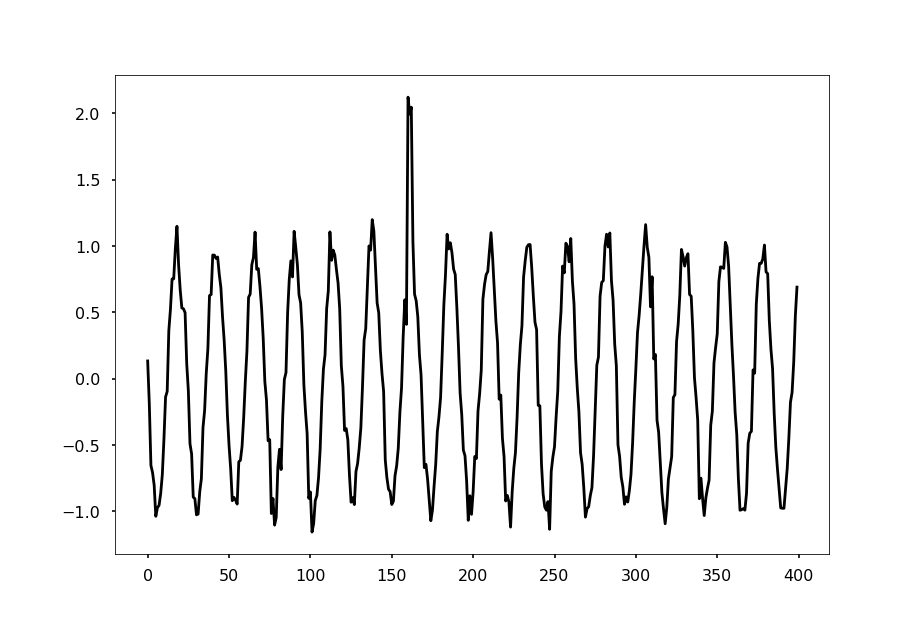
\includegraphics[scale=0.10]{images/local_cp}
		\textbf{Global change point}\par\medskip
		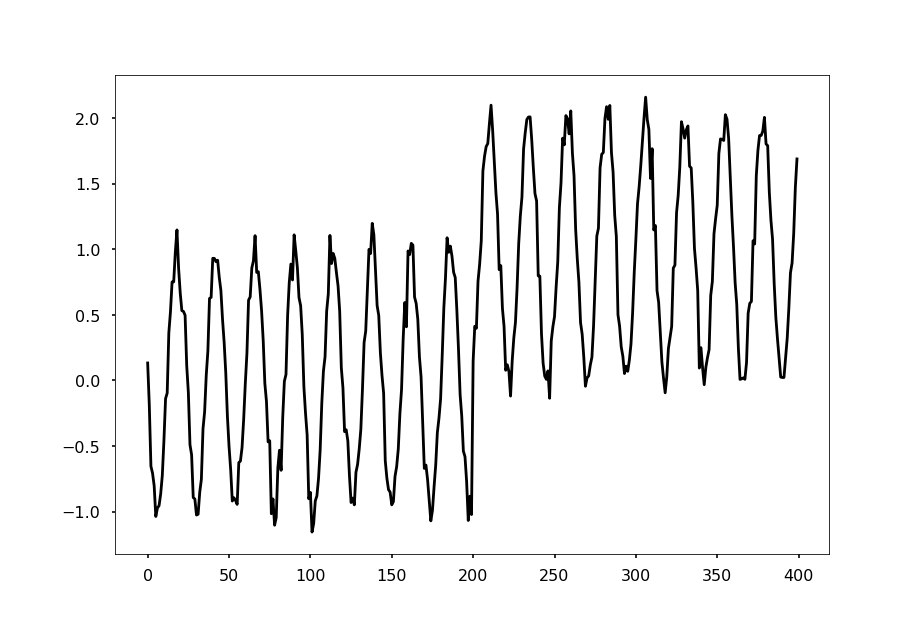
\includegraphics[scale=0.10]{images/global_cp}
	\end{figure}
    \end{itemize}
\end{frame}


\begin{frame}
    \frametitle{Why do we care?}
When it helps:
    \begin{itemize}
    	\item Forecasting
	\item Extracting trend more accurately
    	\item Searching issues in historical data 
	\item Reacting on changes quickly
    \end{itemize}
   
	\begin{figure}
		\textbf{Without CP detection}\par\medskip
		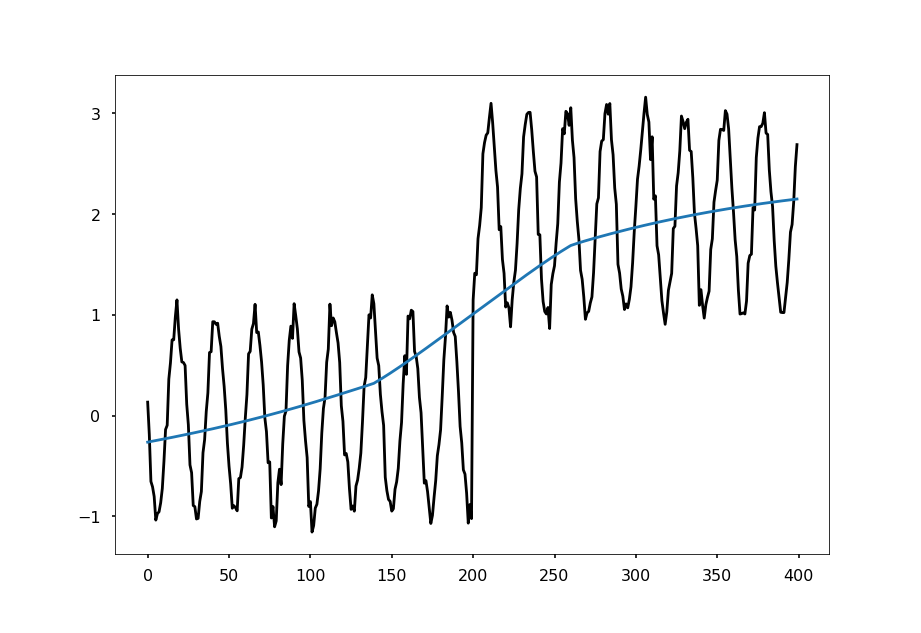
\includegraphics[scale=0.05]{images/trend_fallacy}
		\textbf{With CP detection}\par\medskip
		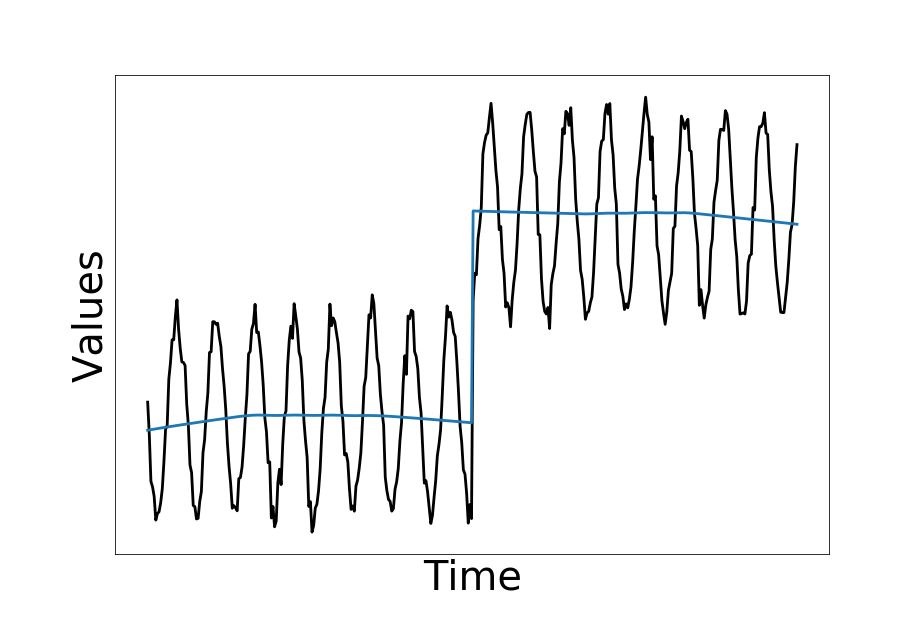
\includegraphics[scale=0.05]{images/trend_succeed}
	\end{figure}
    
What can we do:
    \begin{itemize}
    	\item Remove/change outliers or use robust methods
	\item Split time series and analyze separately
    \end{itemize}

\end{frame}



% \begin{frame}
%     \frametitle{What is change point detection?}
% 
% Let's formalize change point detection problem:
%     \begin{itemize}
% 	\item Suppose $\mathrm{X} = (x_1, ..., x_N)$ --- time series of length $N$
% 	\item $\mathbf{t} = \{t_1,t_2,...\} \subset \{1,...,K\}$ --- set of change points indexes
% 	\item $K-1$ --- amount of changes in time series, which can be either known or unknown
% 	\item Change point detection problem --- is a problem of searching such set of indexes, which would be the closest to real set of change point indexes: $\widehat{\mathbf{t}} = \{\widehat{t_1},\widehat{t_2},...\} $
%  	\item To estimate change point detection algorithm quality we need tagged time series with known indexes $\widehat{\mathbf{t}} = \{\widehat{t_1},\widehat{t_2},...\} $
% 	\item Quality can be estimated as sum of distance between real indexes and estimated indexes normalized by length of time series: $$\sum_{i=1}^K \frac{|\widehat{t_i} - t_i|}{N}$$	
	
%     \end{itemize}
% \end{frame}



\begin{frame}
    \frametitle{Types of change points}


  \begin{columns}[T,onlytextwidth]
      \column{0.5\textwidth}
    \begin{itemize}
    	\item Trend change
	\item Mean change
	\item Variance change
	\item Single point change
	\item Periodic component change
    \end{itemize}

    \column{0.5\textwidth}

	\begin{figure}
		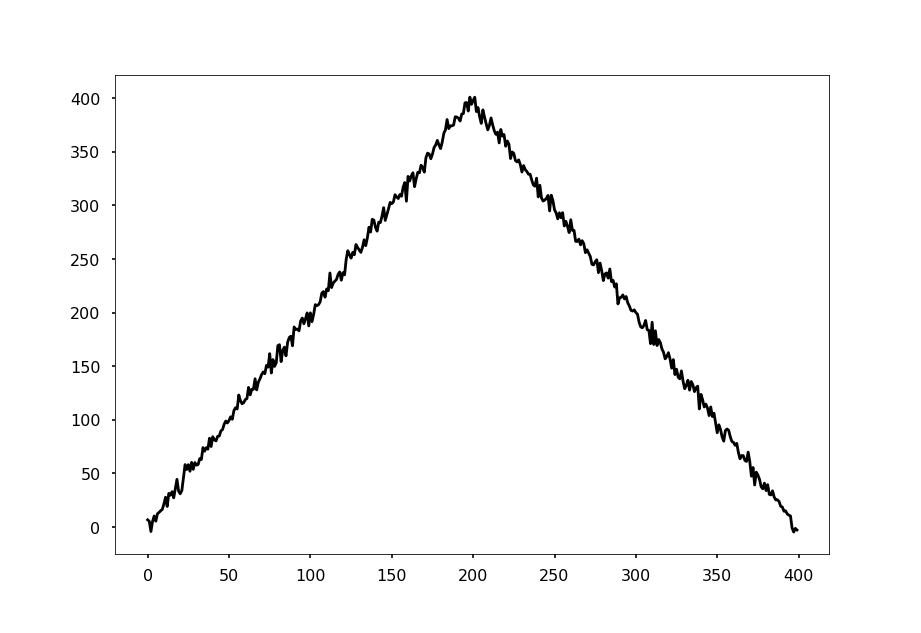
\includegraphics[scale=0.07]{images/examples_trend}
		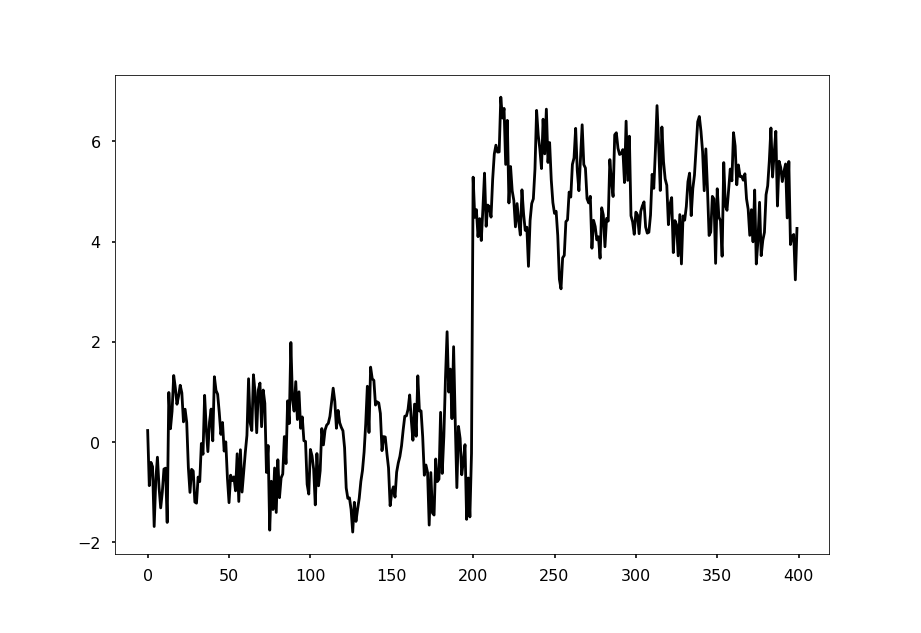
\includegraphics[scale=0.07]{images/examples_mean}
		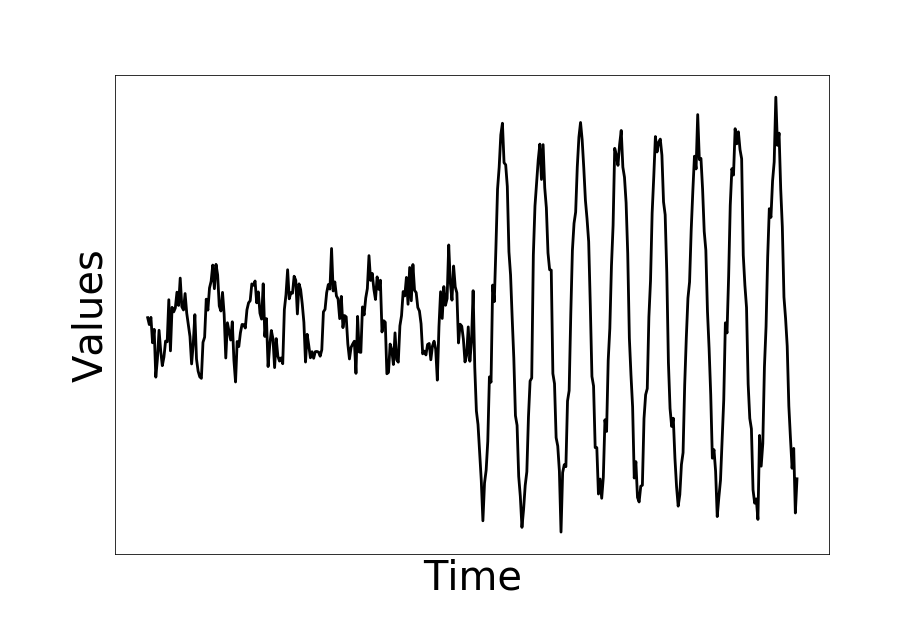
\includegraphics[scale=0.07]{images/examples_variance}
		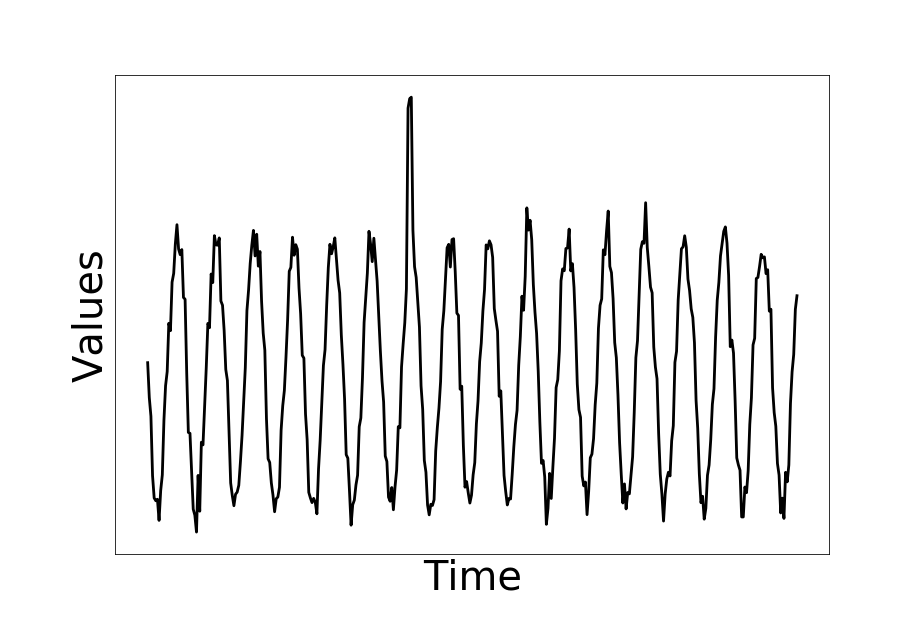
\includegraphics[scale=0.07]{images/examples_outlier}
		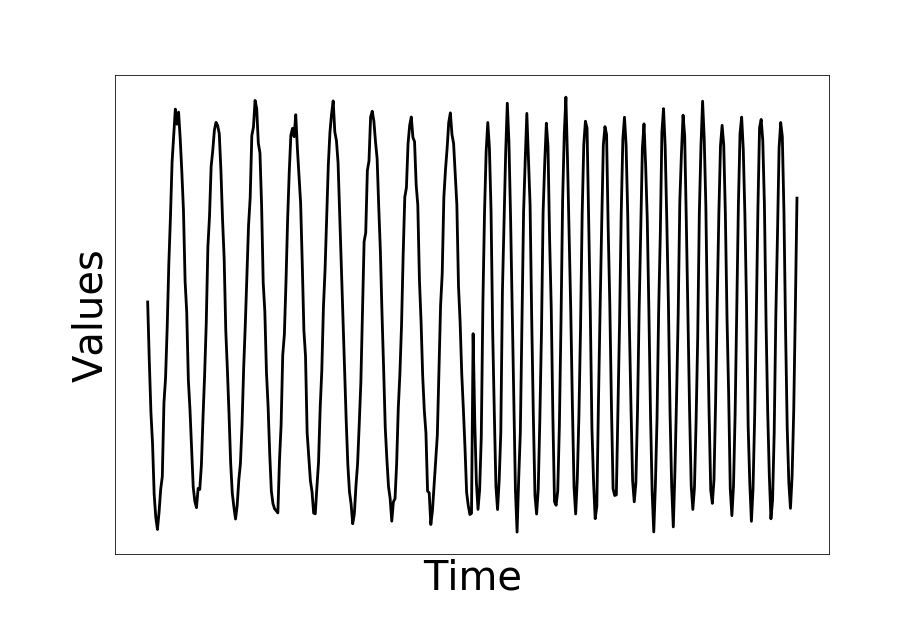
\includegraphics[scale=0.07]{images/examples_periodic}
	\end{figure}

     \end{columns}


\end{frame}

\begin{frame}
\frametitle{Change point examples}
\begin{figure}
\textbf{Common graph}\par\medskip
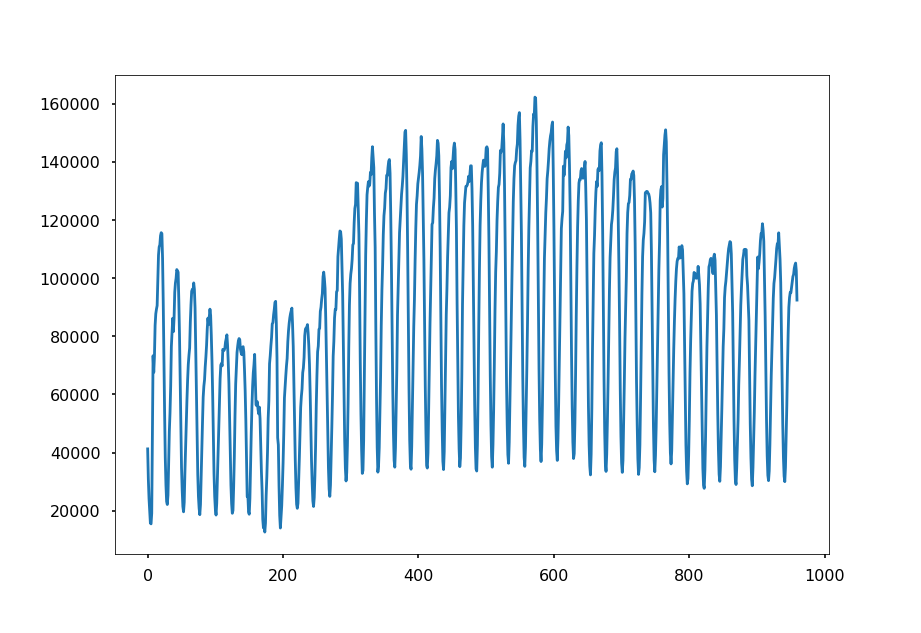
\includegraphics[scale=0.30]{images/001_normal_1}
\end{figure}
\end{frame}

\begin{frame}
\frametitle{Change point examples}
\begin{figure}
\textbf{Common graph with trend}\par\medskip
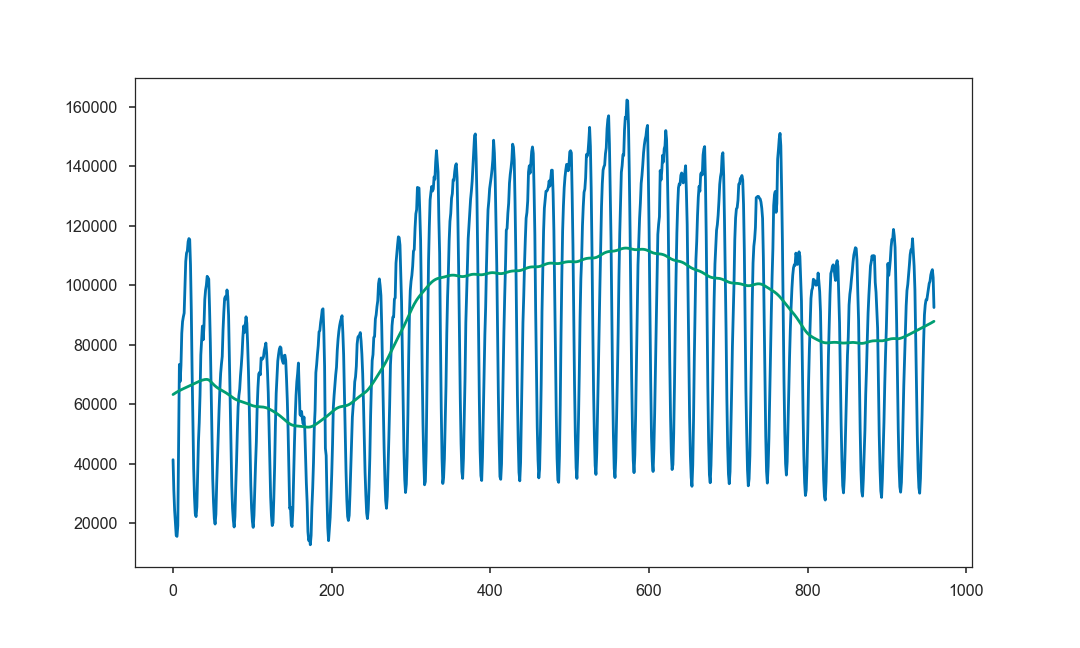
\includegraphics[scale=0.30]{images/001_normal_2}
\end{figure}
\end{frame}

\begin{frame}
\frametitle{Change point examples}
\begin{figure}
\textbf{Common graph without trend}\par\medskip
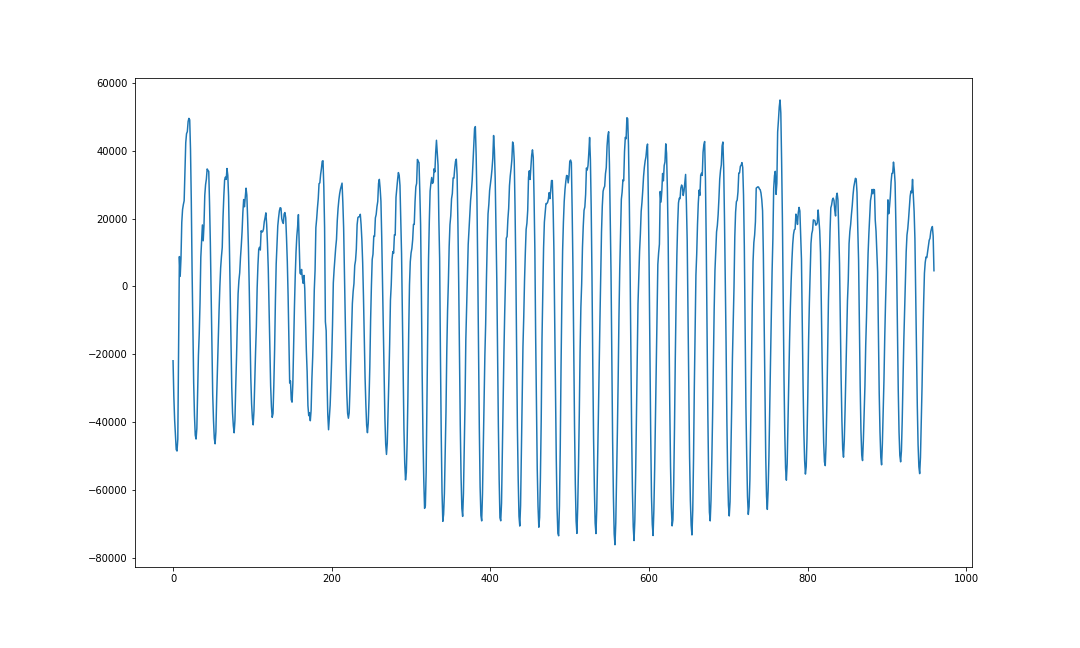
\includegraphics[scale=0.30]{images/001_normal_3}
\end{figure}
\end{frame}

\begin{frame}
\frametitle{Change point examples}
\begin{figure}
\textbf{Common graph periodic frequency}\par\medskip
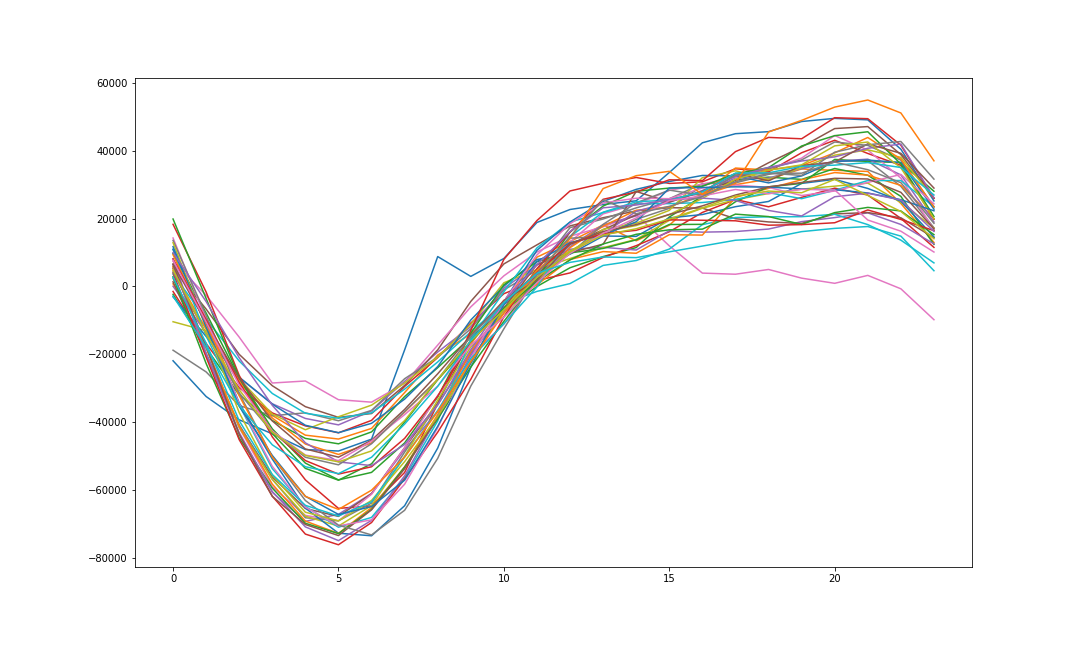
\includegraphics[scale=0.30]{images/001_normal_4}
\end{figure}
\end{frame}

\begin{frame}
\frametitle{Change point examples}
\begin{figure}
\textbf{Mean change}\par\medskip
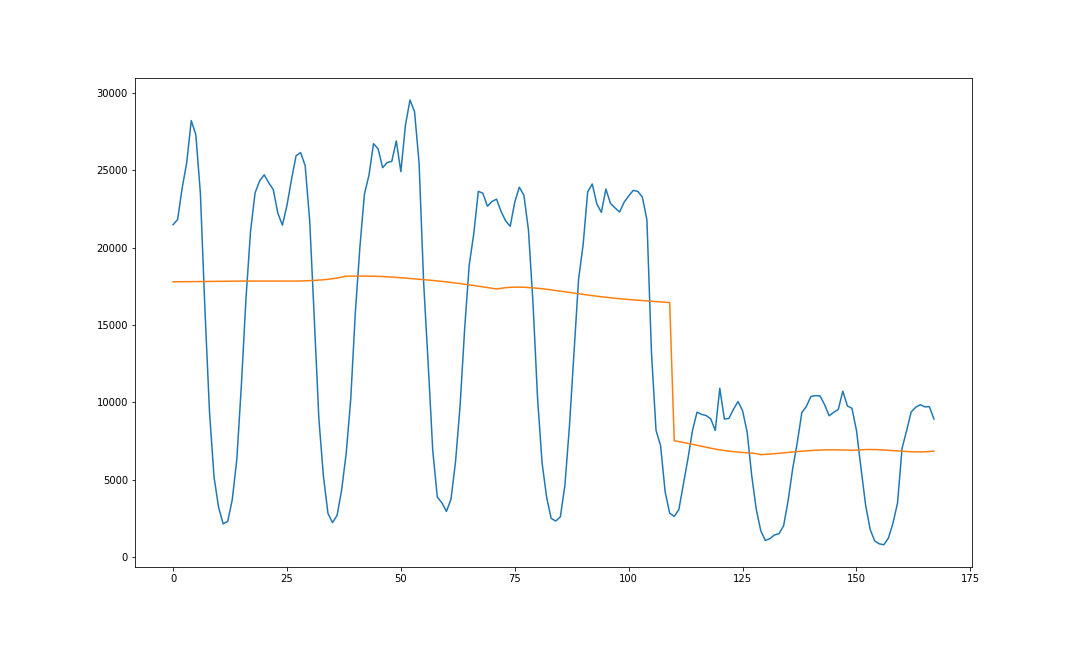
\includegraphics[scale=0.30]{images/002_mean}
\end{figure}
\end{frame}

\begin{frame}
\frametitle{Change point examples}
\begin{figure}
\textbf{Variance change}\par\medskip
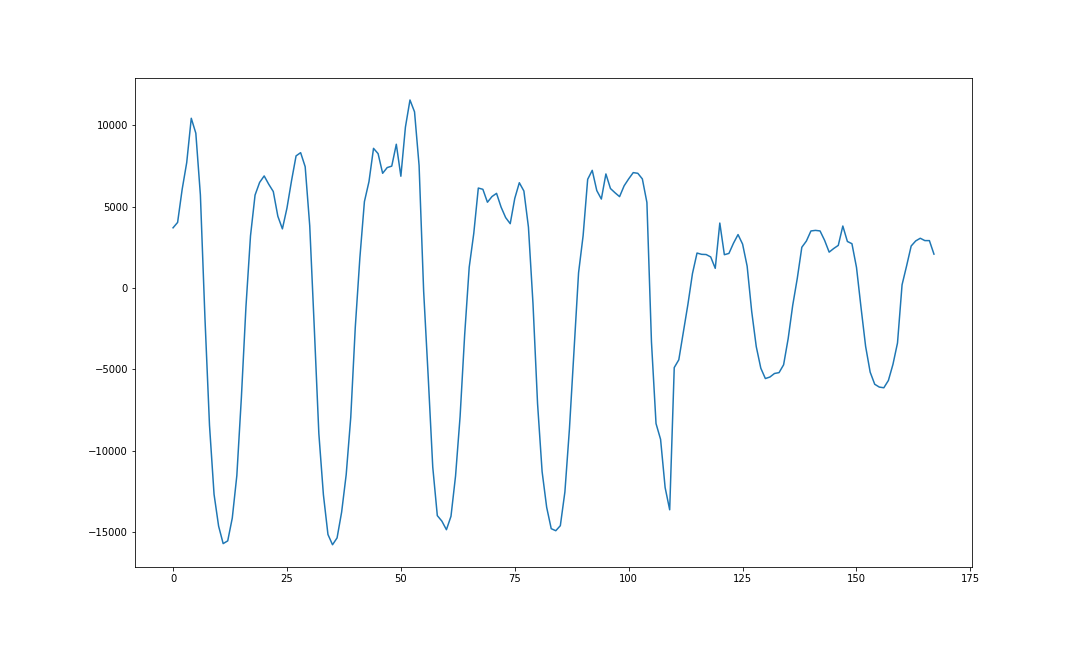
\includegraphics[scale=0.30]{images/003_variance}
\end{figure}
\end{frame}

\begin{frame}
\frametitle{Change point examples}
\begin{figure}
\textbf{Trend change}\par\medskip
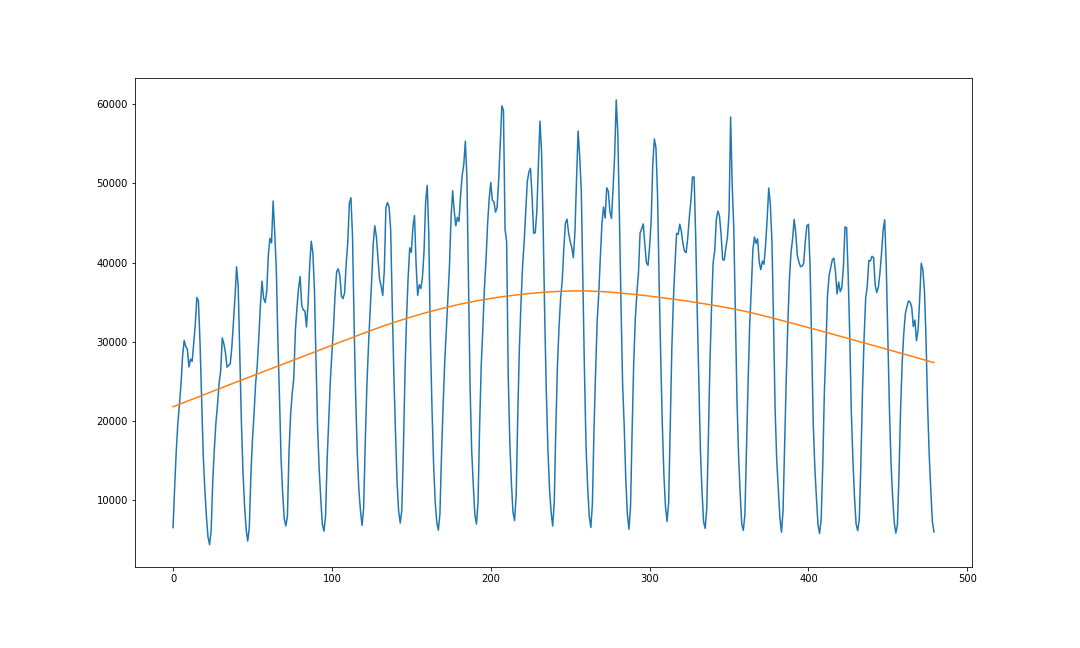
\includegraphics[scale=0.30]{images/004_trend}
\end{figure}
\end{frame}

\begin{frame}
\frametitle{Change point examples}
\begin{figure}
\textbf{Point change}\par\medskip
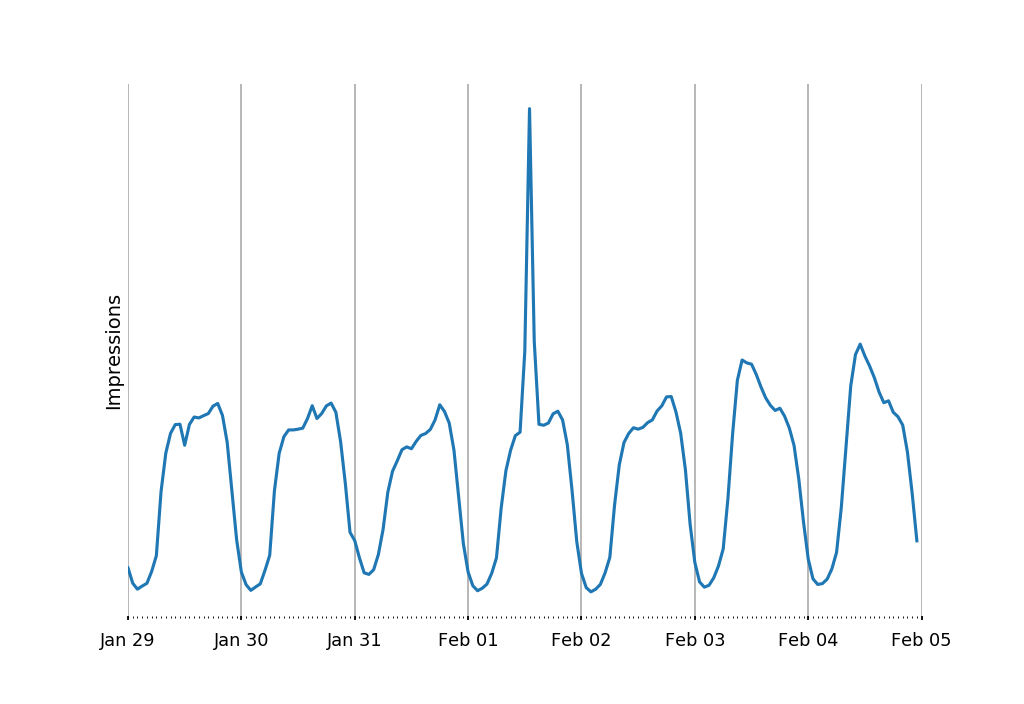
\includegraphics[scale=0.30]{images/005_point}
\end{figure}
\end{frame}

\begin{frame}
\frametitle{Change point examples}
\begin{figure}
\textbf{Structure change}\par\medskip
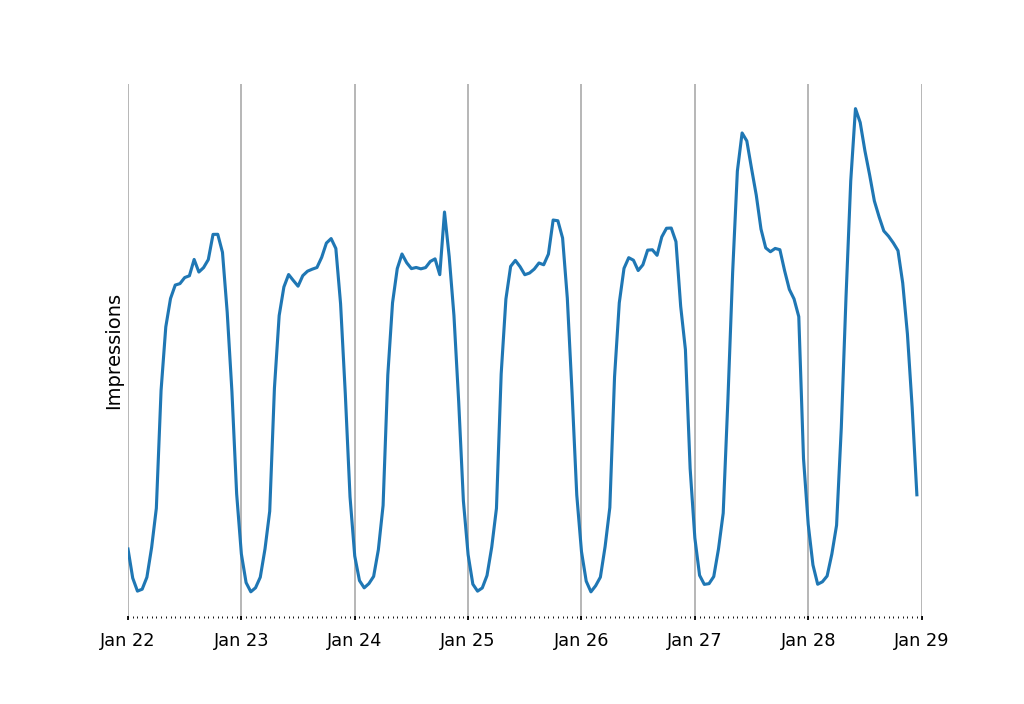
\includegraphics[scale=0.30]{images/006_structure}
\end{figure}
\end{frame}


\section{Change point detection techniques}

\begin{frame}
    \frametitle{SSA for change point detection}

Singular spectrum analysis (SSA) method can be used to allocate change points.
Let $x_1,x_2,...$ be a time series and $N, L, l, p, q$ be fixed integers so that $0 \leq l < L \leq N/2$ and $ 0 \leq p < q$. The SSA change point detection algorithm is as follows.
For each $ n = 0,1,...$ we compute:
    \begin{itemize}
    	\item the base matrix $\mathbb{X}^{(n)}$,
	\item the lag-covariance matrix $\mathbb{R}_n = \mathbb{X}^{(n)}(\mathbb{X}^{(n)})^{\top}$,
	\item the SVD of $\mathbb{R}_n$,
	\item $\mathbf{\nu}_{n.I,p,q}$, the sum of the squared Euclidean distances between the vectors $\mathbb{X}_j^{(n)} (j = p+1,...,q$ and the l-dimensional subspace $L_{n,I}$, and
	\item $S_n$, the normalized squared distance.
    \end{itemize}
 Large values of $S_n$ indicate a change in the time series.

This method has the following parameters:
	\begin{itemize}
		\item $N$ --- window size for base matrix
		\item $L, I$ --- SSA window and number of eigenvectors
		\item $p, q$ --- window size for test matrix
		\item threshold
	\end{itemize}
\end{frame}

\begin{frame}
    \frametitle{SSA in action. Mean change}

Let's try to apply SSA algorithm to real time series mentioned above. With manually settled parameters.
\begin{figure}
	\textbf{Mean change}
	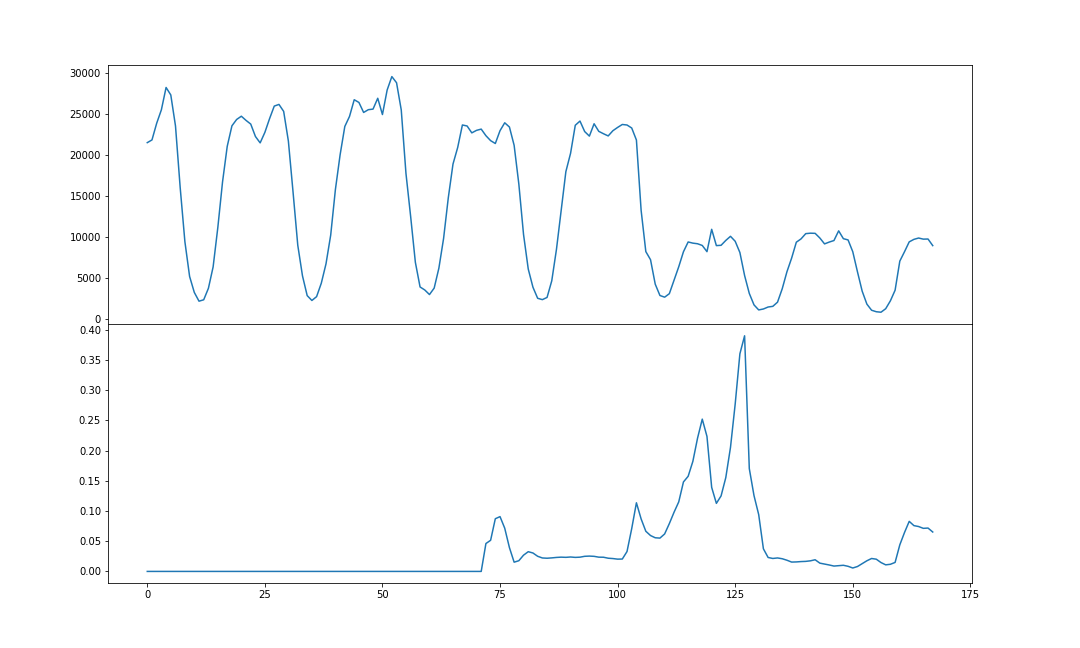
\includegraphics[scale=0.10]{images/017_mean_cp}
	\textbf{Detection}
	N = 48, L = 24, I = 5, p = 49, q = L, threshold = 0.15
	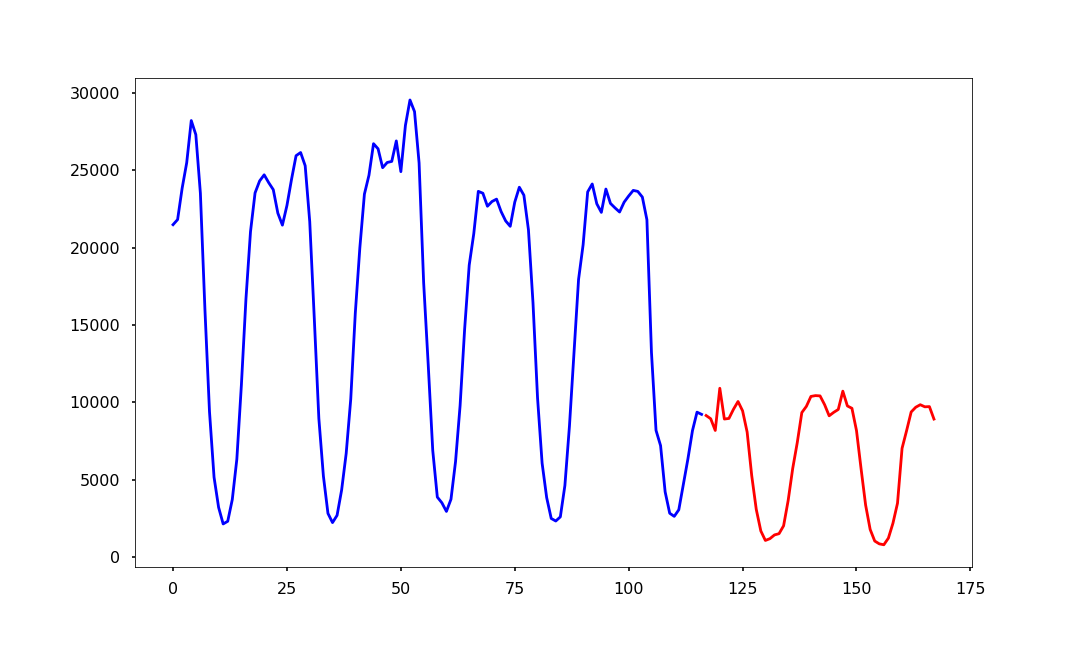
\includegraphics[scale=0.10]{images/018_mean_cp_detected}
\end{figure}

Works good for mean change

\end{frame}

\begin{frame}
    \frametitle{SSA in action. Variance change}

\begin{figure}
	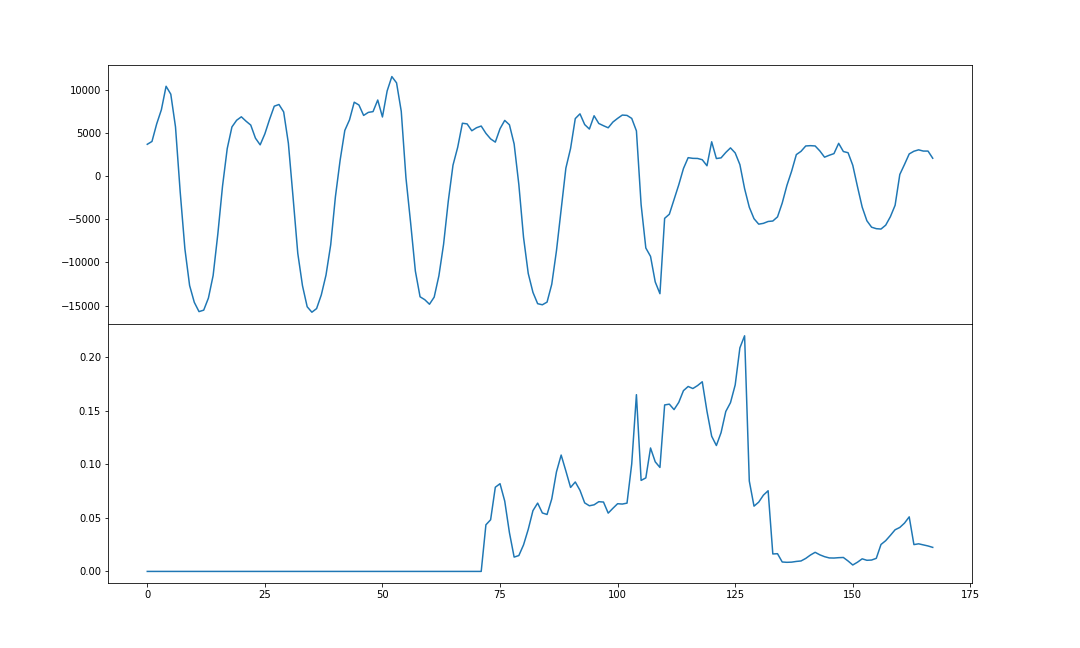
\includegraphics[scale=0.10]{images/019_variance_cp}
	N = 48, L = 24, I = 5, p = 49, q = L, threshold = 0.15
	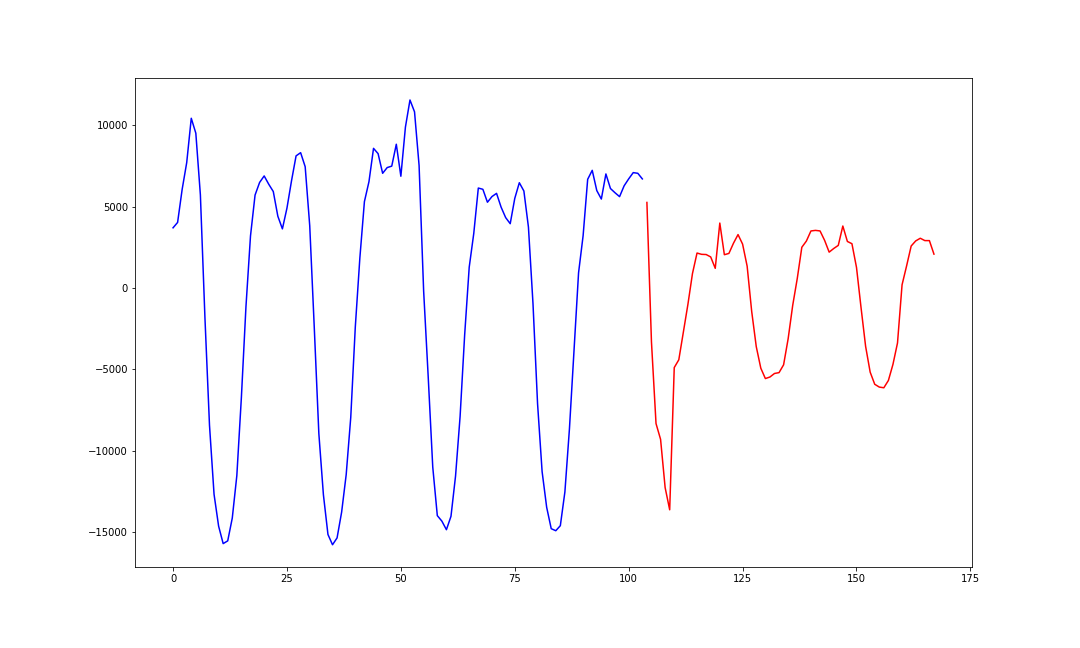
\includegraphics[scale=0.10]{images/020_variance_cp_detected}
\end{figure}

Works good for variance change

\end{frame}

\begin{frame}
    \frametitle{SSA in action. Period change}

\begin{figure}
	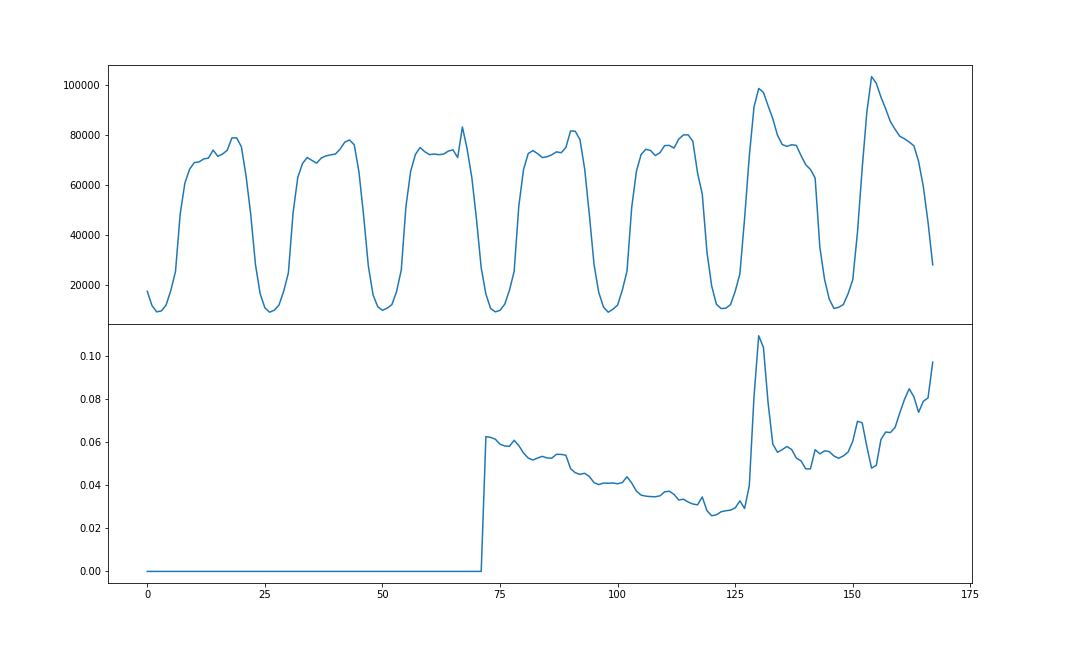
\includegraphics[scale=0.10]{images/025_period_cp}
	N = 48, L = 24, I = 5, p = 49, q = L, threshold = 0.1
	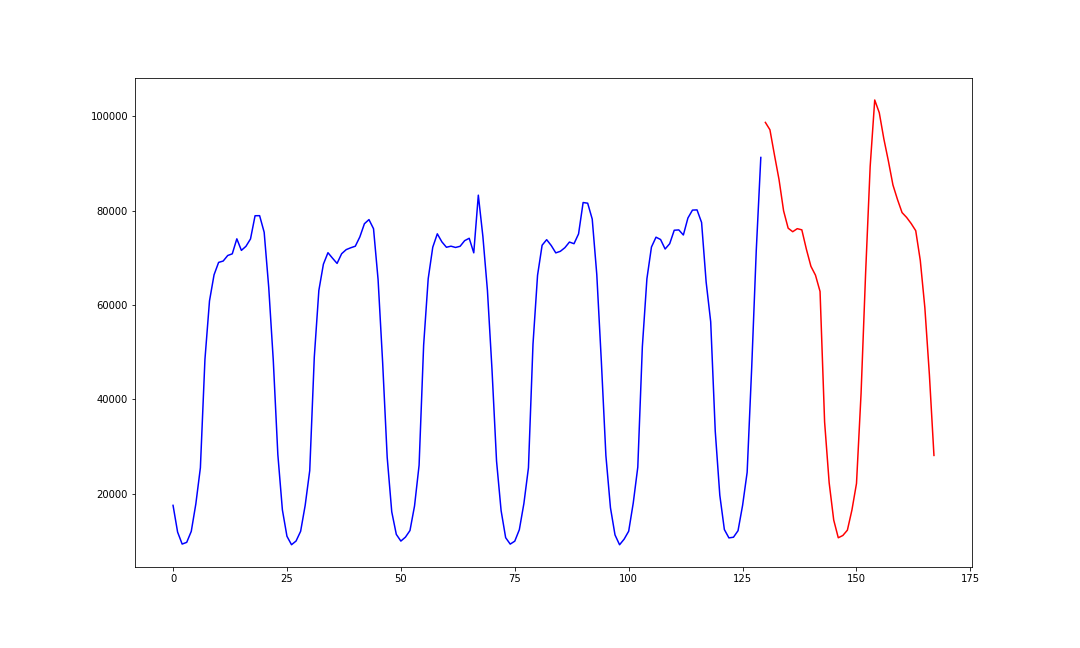
\includegraphics[scale=0.10]{images/026_period_cp_detected}
\end{figure}

Works well for period change

\end{frame}


\begin{frame}
    \frametitle{SSA in action. Point change}

\begin{figure}
	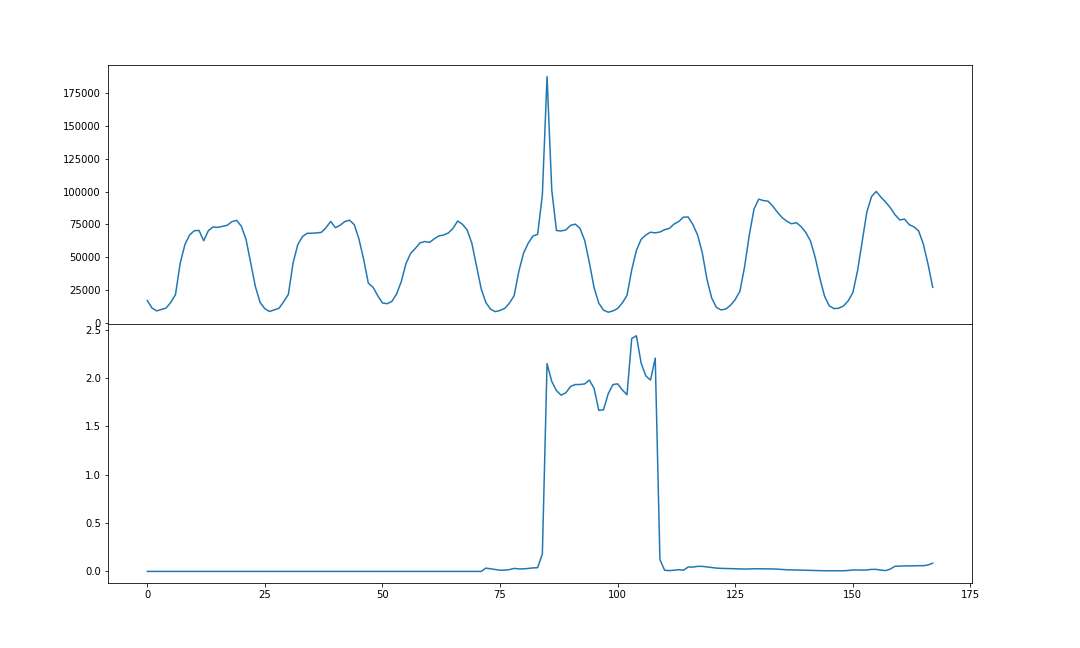
\includegraphics[scale=0.10]{images/021_point_cp}
	N = 48, L = 24, I = 5, p = 49, q = L, threshold = 0.1
	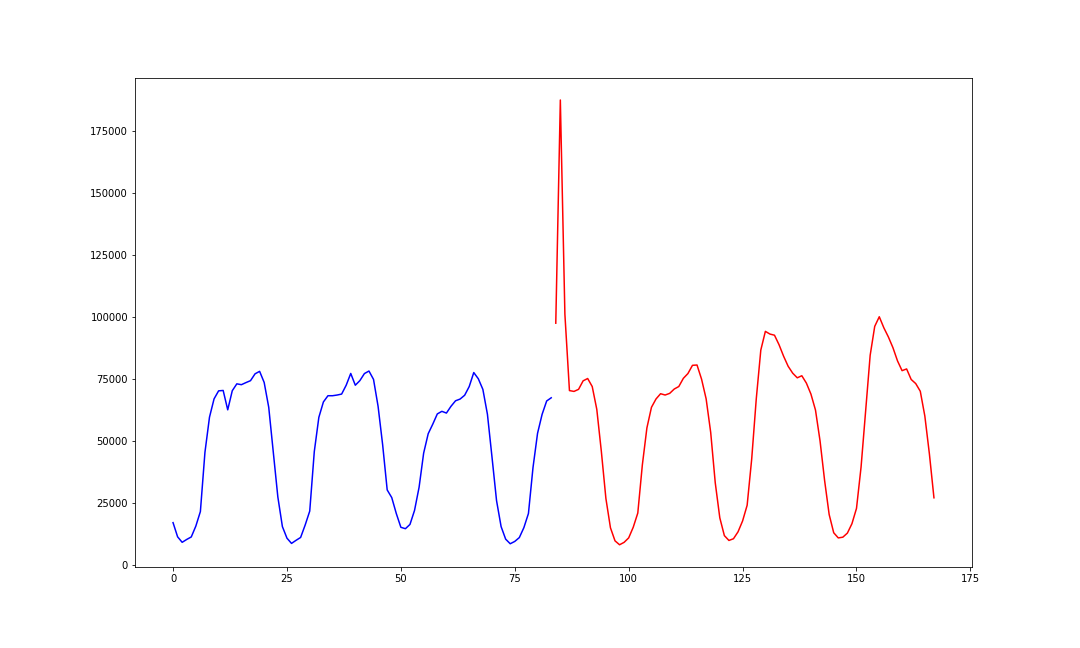
\includegraphics[scale=0.10]{images/022_point_cp_detected}
\end{figure}

Doesn't work for point change.
The reason is that we always move window from left to the right.

\end{frame}

\begin{frame}
    \frametitle{SSA in action. Point change}
    
Let's try to reverse the time series each time we find change point.

\begin{figure}
	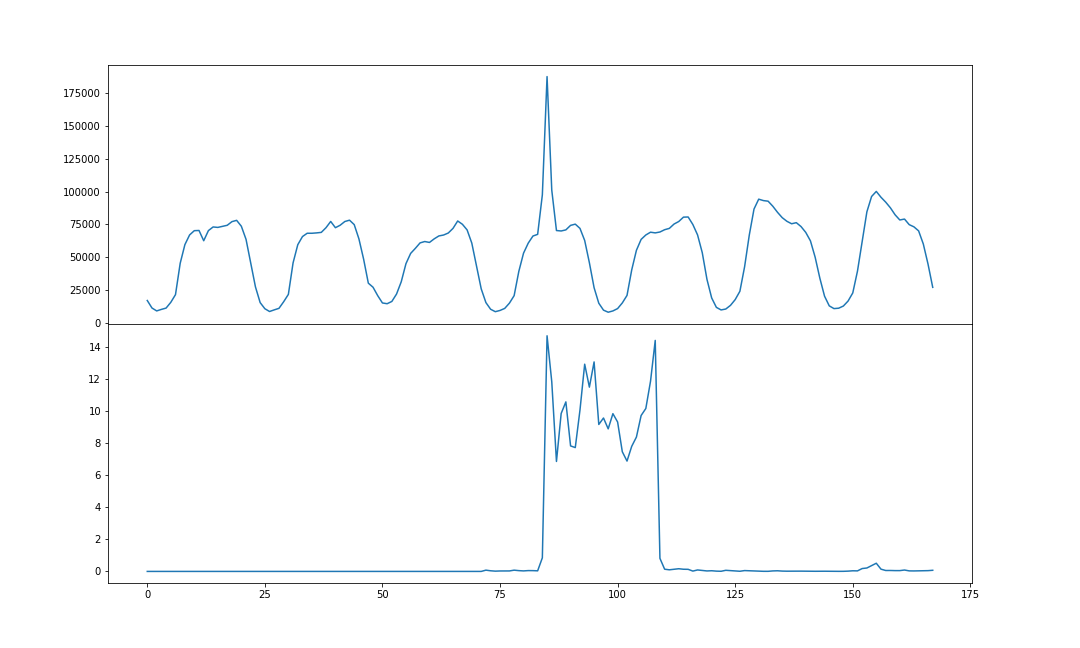
\includegraphics[scale=0.10]{images/023_point_cp_2}
	N = 48, L = 24, I = 5, p = 49, q = L, threshold = 0.1
	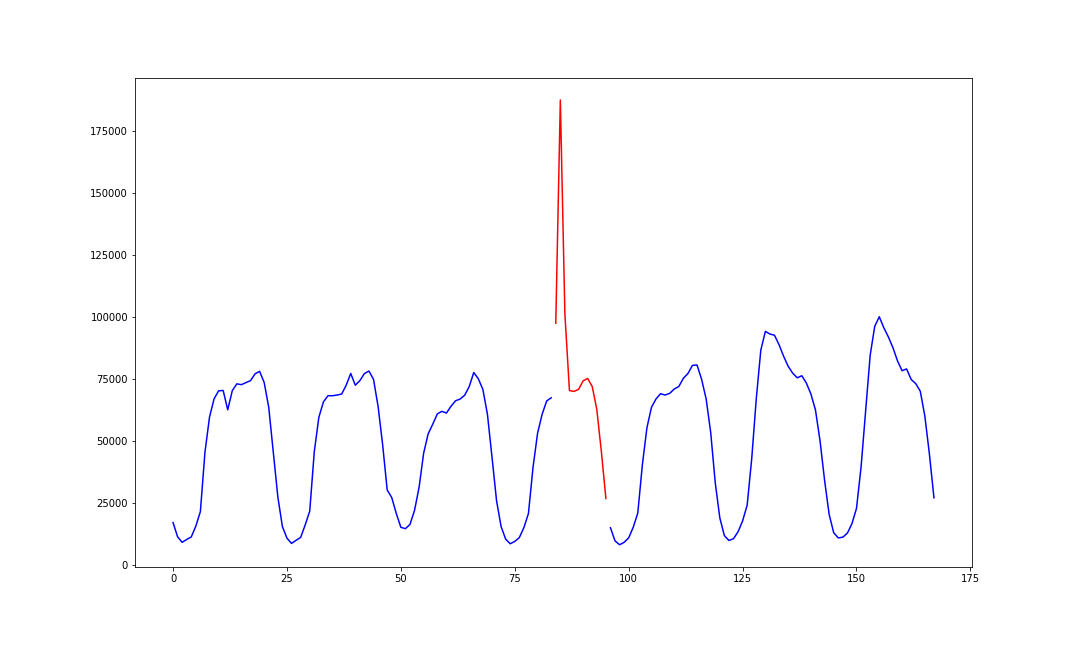
\includegraphics[scale=0.10]{images/024_point_cp_detected_2}
\end{figure}

Using this upgrade we make SSA algorithm working for point change as well

\end{frame}


\begin{frame}
    \frametitle{Long time series}

	\begin{itemize}
		\item We have 5 time series 2856 points each. It is impressions time series for different countries hourly for 17 weeks.
		\item We have tagged change points manually in all these time series
	\end{itemize}

\end{frame}


\begin{frame}
    \frametitle{Country A}
\begin{figure}
	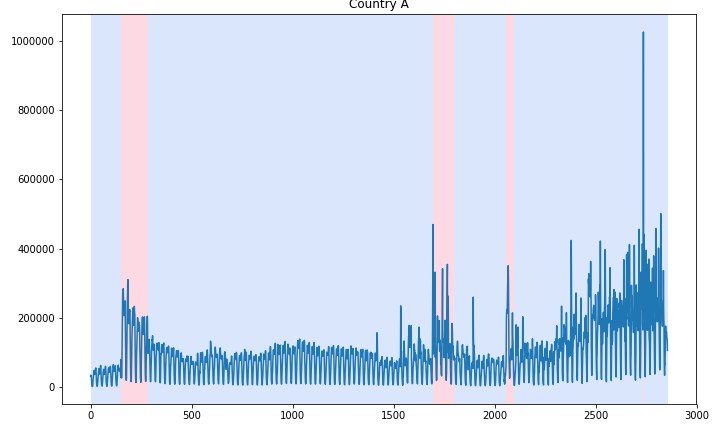
\includegraphics[scale=0.30]{images/028_country_a}
	In time series for Country A we manually detected 6 change points. First one - mean change along with variance change. Second one - variance change. Third one - point change. Fourth one - variance change. Fifth and sixth - points change.
\end{figure}
\end{frame}

\begin{frame}
    \frametitle{Country B}
\begin{figure}
	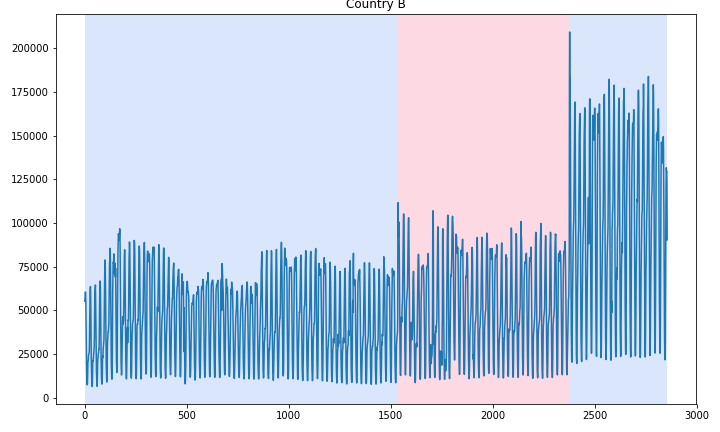
\includegraphics[scale=0.30]{images/029_country_b}
	In time series for Country B we manually detected 2 change points. First one - mean change along with variance change. Second one - mean change along with variance change.
\end{figure}
\end{frame}

\begin{frame}
    \frametitle{Country C}
\begin{figure}
	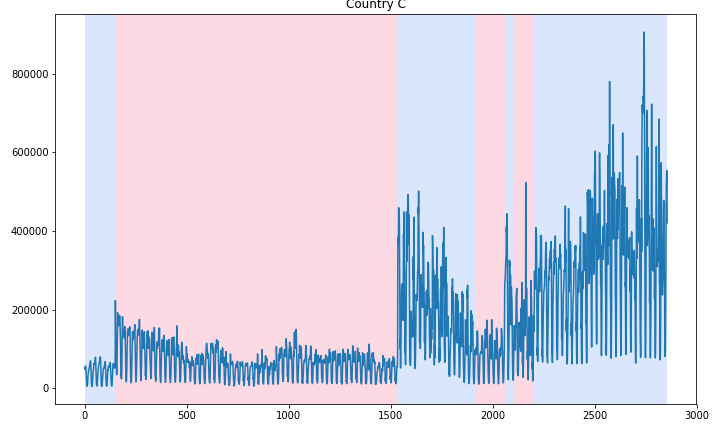
\includegraphics[scale=0.30]{images/030_country_c}
	In time series for Country C we manually detected 5 change points. First, second and fifth - mean change along with variance change (similar to country A). Third - variance change. Fourth - point change
\end{figure}
\end{frame}

\begin{frame}
    \frametitle{Country D}
\begin{figure}
	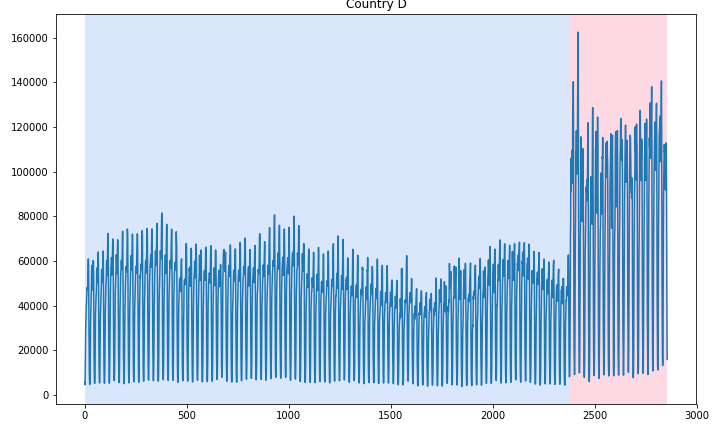
\includegraphics[scale=0.30]{images/031_country_d}
	In time series for Country D only one change point was manually detected - mean change along with variance change.
\end{figure}
\end{frame}

\begin{frame}
    \frametitle{Country E}
\begin{figure}
	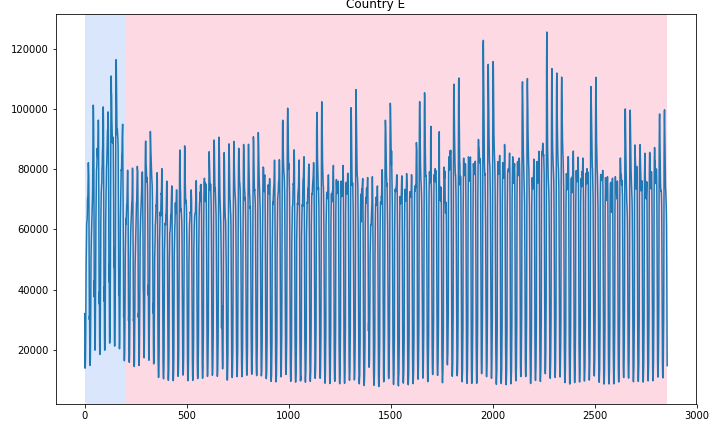
\includegraphics[scale=0.30]{images/032_country_e}
	In time series for Country E there is only one change point - mean change.
\end{figure}
\end{frame}




\begin{frame}
    \frametitle{Another change point detection approach}
	
	\begin{itemize}
		\item Apart from SSA there is another approach to find change points
		\item We can define change point detection problem as minimizing contrast function:
		$$ \mathbb{V}(\mathbf{t},\mathrm{X}) := \sum_{i=1}^K c(x_{t_i}...x_{t+1}) $$, where $c()$ --- some cost function, and $x_{t_i}...x_{t+1}$ --- sub series of initial time series
		\item When quantity of change points $K$ is known the problem is:
		$$ \min_t{\mathbb{V}(\mathbf{t},\mathrm{X})} $$
		\item When quantity of change points unknown, then additional parameter penalty is added:
		$$ \min_t{\mathbb{V}(\mathbf{t},\mathrm{X})} + pen(\mathbf{t},\mathrm{X}) $$
	\end{itemize}

Thus, such approach can be described as follows steps:

	\begin{itemize}
		\item Choosing cost function
		\item Minimizing contrast function
		\item Searching for change points quantity (when unknown beforehand)
	\end{itemize}
\end{frame}


\begin{frame}
    \frametitle{Cost functions}
	
	There could be plenty of cost functions. Let's describe the most popular
	\begin{itemize}
		\item Mean absolute deviation. It finds changes in medians.
		$$ c(\mathbf{X}_I) = \sum_{t \in I}||\mathbf{X}_t - \bar{\mathbf{X}} ||_1 $$
		\item Mean squared deviation. It finds changes in means.
		$$ c(\mathbf{X}_I) = \sum_{t \in I}||\mathbf{X}_t - \bar{\mathbf{X}} ||_2^2 $$
		\item Kernel based method
		$$ c(\mathbf{X}_I) = \sum_{t\in I} ||\Phi (\mathbf{X}_t) - \bar{\mu} ||_{\mathcal{H}}^2 $$
		\item Autoregression
		$$ c(\mathbf{X}_I) = \min_{\delta \in \mathbb{R}_p}\sum||\mathbf{X}_t - \delta'z_t||_2^2 $$
	\end{itemize}


\end{frame}


\begin{frame}
    \frametitle{Cost functions. Continue}
	
	We can also create our own cost function.
	Fore example, according to understanding of our time series we can assume that it can be described with such model:
	$$ \mathrm{X} = a + C\cos(2\pi \frac{n}{24}) + S \sin(2\pi \frac{n}{24}) + \epsilon $$
	Then cost function can be:
	$$ c(\mathbf{X}_I) = \sum_{t \in I}||\mathbf{X}_t - (a + C\cos(2\pi \frac{n}{24}) + S \sin(2\pi \frac{n}{24})) ||_2^2 $$
\end{frame}

\begin{frame}
    \frametitle{Search method}
	
	Apart from cost function we need to choose method of search change points.
	There are several well researched methods, we will use one of them --- window method.
	Idea is straightforward: 
	\begin{itemize}
		\item Choosing wide of the window $w$
		\item Then algorithm slides across the time series with this window
		\item On each iteration it splits time series into two sub series
		\item Then for each sub series special metric is calculated:
		$$ d(x_{u..v},x_{v..w}) = c(x_{u..w}) - c(x_{u..v}) - c(x_{v..w}) $$
	\end{itemize}
	
\end{frame}


\begin{frame}
    \frametitle{Applying approach to the real data}
	
	Let's try to apply all of the mentioned cost functions to the time series described above
	\begin{table}[]
\begin{tabular}{llllll}
          & custom function & L1     & L2     & RBF    & Autoregression \\
Country A & 1.3582          & 0.2507 & 1.305  & 0.6877 & 2.3939         \\
Country B & 0.3312          & 0.0942 & 0.3312 & 0.8267 & 0.4111         \\
Country C & 1.2686          & 0.3407 & 1.1478 & 0.4265 & 1.6971         \\
Country D & 0.0007          & 0.0007 & 0.0007 & 0.0011 & 0.0025         \\
Country E & 0.4982          & 0.013  & 0.7521 & 0.0042 & 0.3022        
\end{tabular}
\end{table}

The best result shows $L_1$ cost function (mean absolute deviation).
	
\end{frame}

\begin{frame}
    \frametitle{Applying approach to the real data. Contine}
	
	Let's take a look on the data
\begin{figure}
	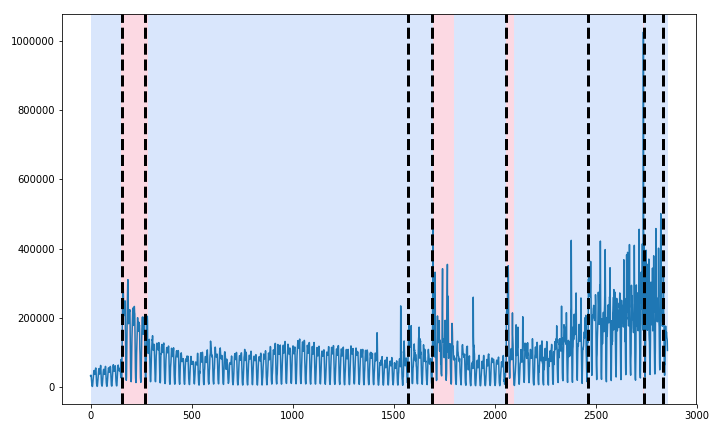
\includegraphics[scale=0.10]{images/033_country_a_cp}
	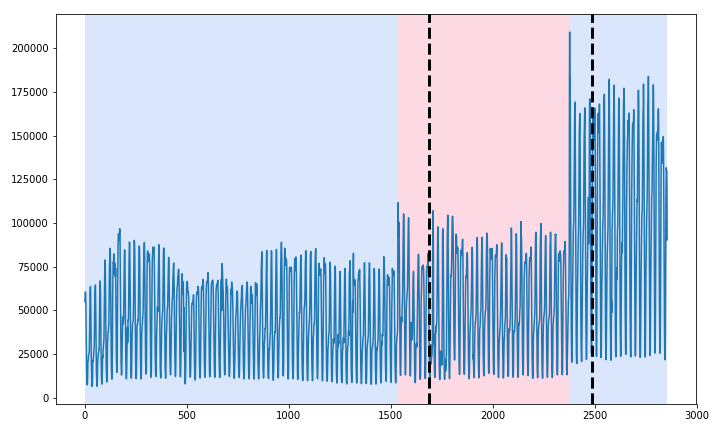
\includegraphics[scale=0.10]{images/034_country_b_cp}
	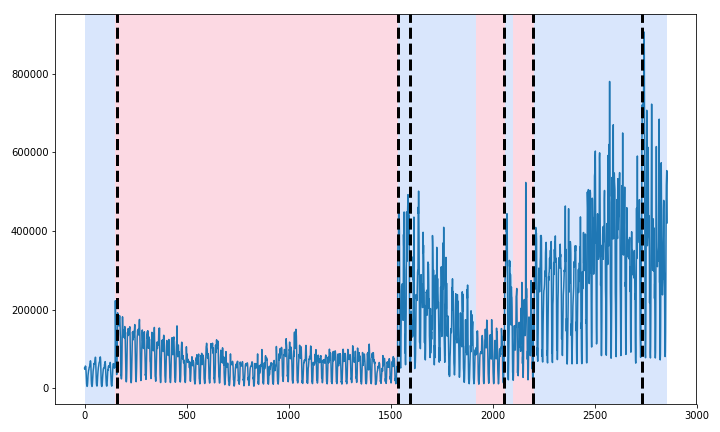
\includegraphics[scale=0.10]{images/035_country_c_cp}
	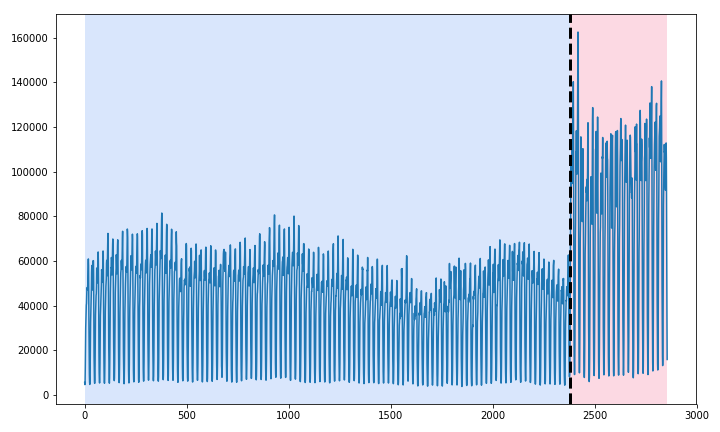
\includegraphics[scale=0.10]{images/036_country_d_cp}
	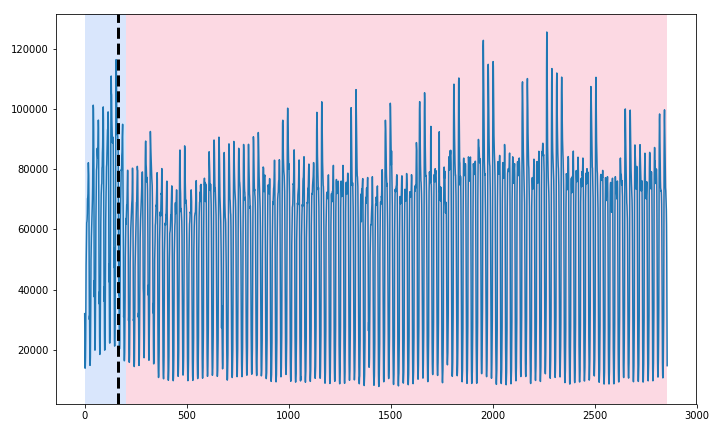
\includegraphics[scale=0.10]{images/037_country_e_cp}
\end{figure}

Most of the time looks pretty good.
\end{frame}

\begin{frame}
    \frametitle{Applying approach to the real data. Contine}
	
	Above case was when we defined number of change points in advance. But in real life problems most of the time do not know it.
	Thus let's try to calculate quantity of change points, using following penalty function:
	$$ pen_{BIC, L_2}(t) := \sigma \log{T}, $$
	Here is the results on number of change points:
	
	Country A --- Actual amount: 8; Predicted amount: 5 
	
	Country B  --- Actual amount: 2; Predicted amount: 2 
	
	Country C --- Actual amount: 6; Predicted amount: 6 

	Country D --- Actual amount: 1; Predicted amount: 2 
	
	Country E --- Actual amount: 1; Predicted amount: 1 
	
\end{frame}


\section{Airpush cases}

\begin{frame}
    \frametitle{Airpush cases. Fraud elimination}
    \begin{itemize}
    	\item Apps minutely requests data
	\item Red flag: strong pattern.
	\item Can be a automated bots behind pattern
    \end{itemize}
    \begin{figure}
	\textbf{Clean application}
	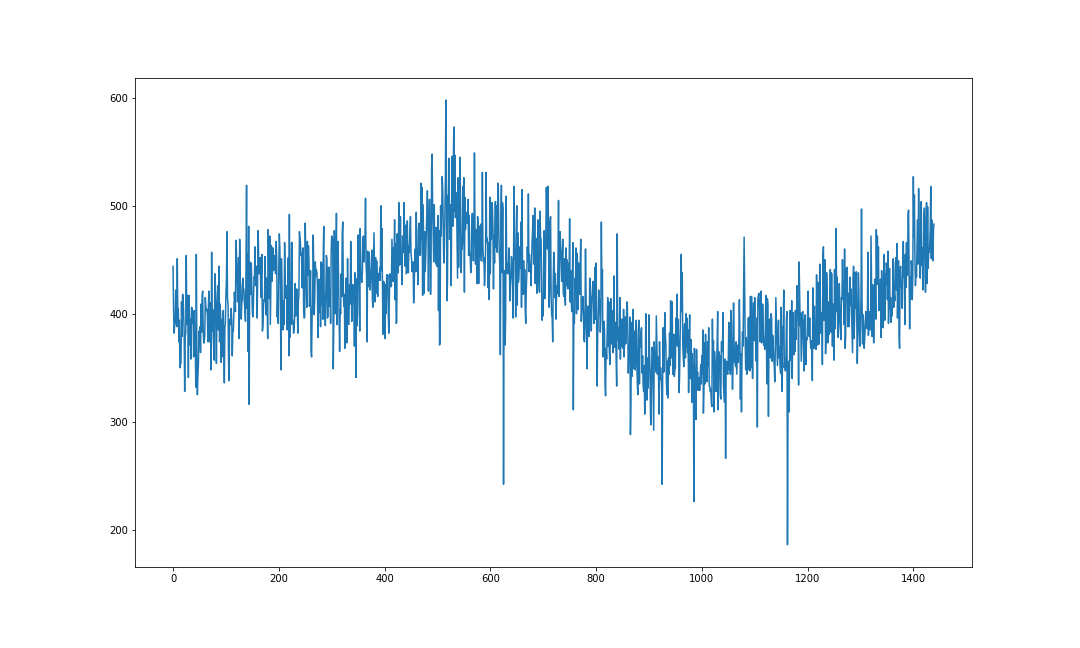
\includegraphics[scale=0.10]{images/007_case_1}
	\textbf{Fraud application}
	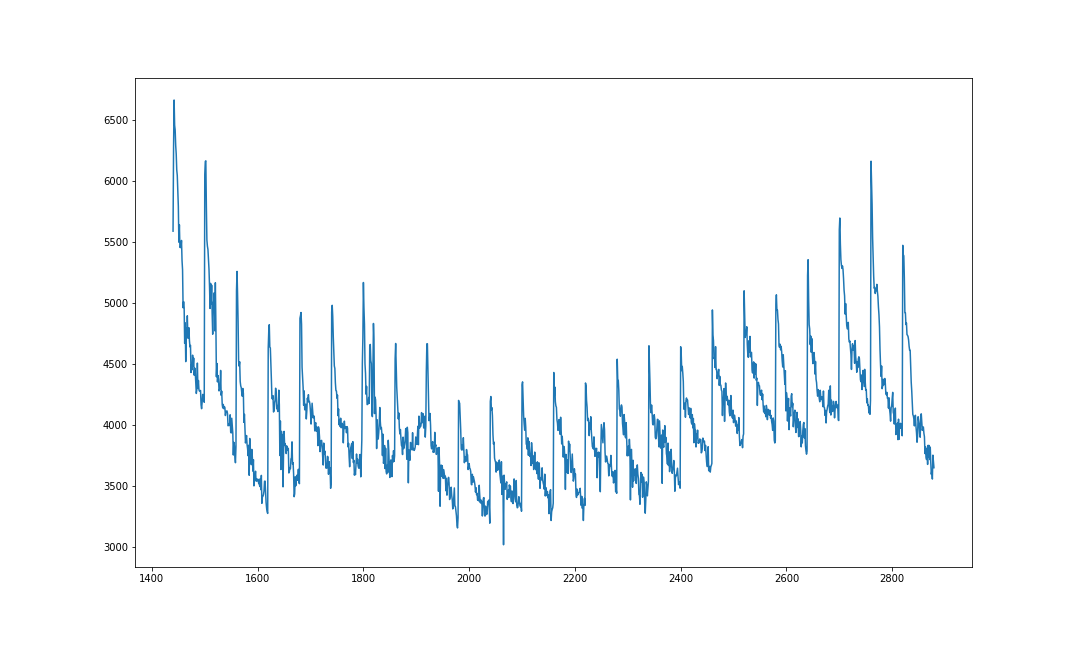
\includegraphics[scale=0.10]{images/008_case_1}
     \end{figure}
	
\end{frame}


\begin{frame}
    \frametitle{Airpush cases. Fraud elimination}
    \begin{itemize}
    	\item Goal: to be able to find such apps automatically
	\item We can reach this goal using frequency analysis
    \end{itemize}
    The framework can be described as follows:
   	 \begin{enumerate}
	 \item Apply logarithm to time series to stabilyze amplitude
 	 \item Remove trend (low frequent part) from time series
	 \item Apply Fourier transform to time series
	 \item Estimate the distribution of periodogram values
	 \item Compare distributions of each application with a distribution of white noise (which is exponential) using Kullback–Leibler divergence 
	 \item If divergence $>$ threshold, then application is marked as suspicious
	\end{enumerate}
\end{frame}



\begin{frame}
    \frametitle{Airpush cases. Fraud elimination}
    \framesubtitle{1. Apply logarithm}
    \begin{figure}
	\textbf{Clean application}
	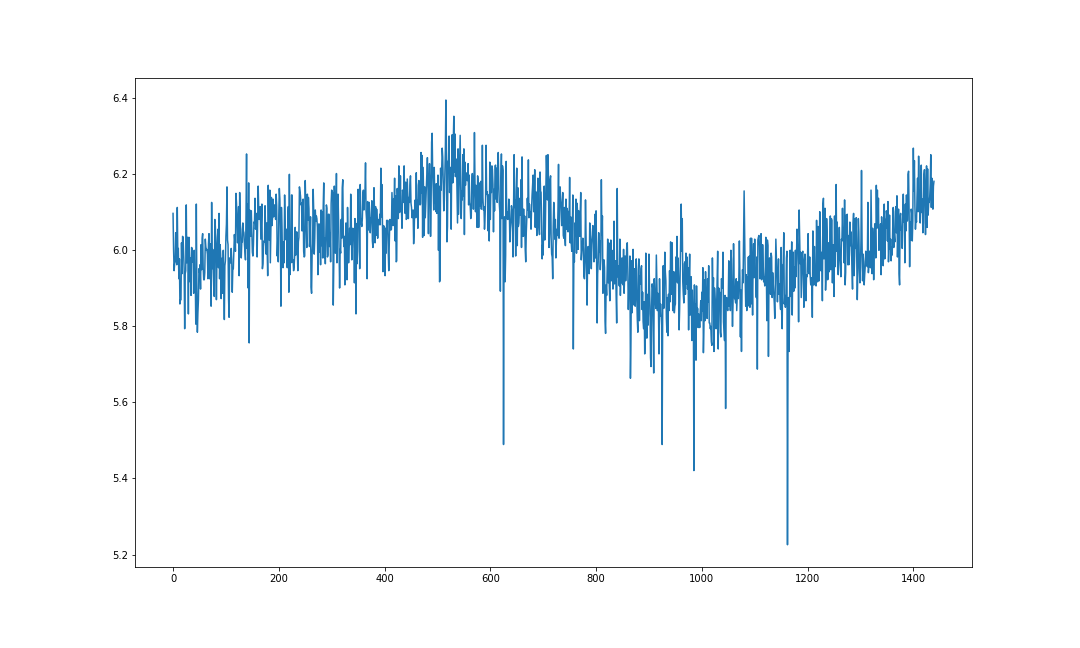
\includegraphics[scale=0.10]{images/009_case_1}
	\textbf{Fraud application}
	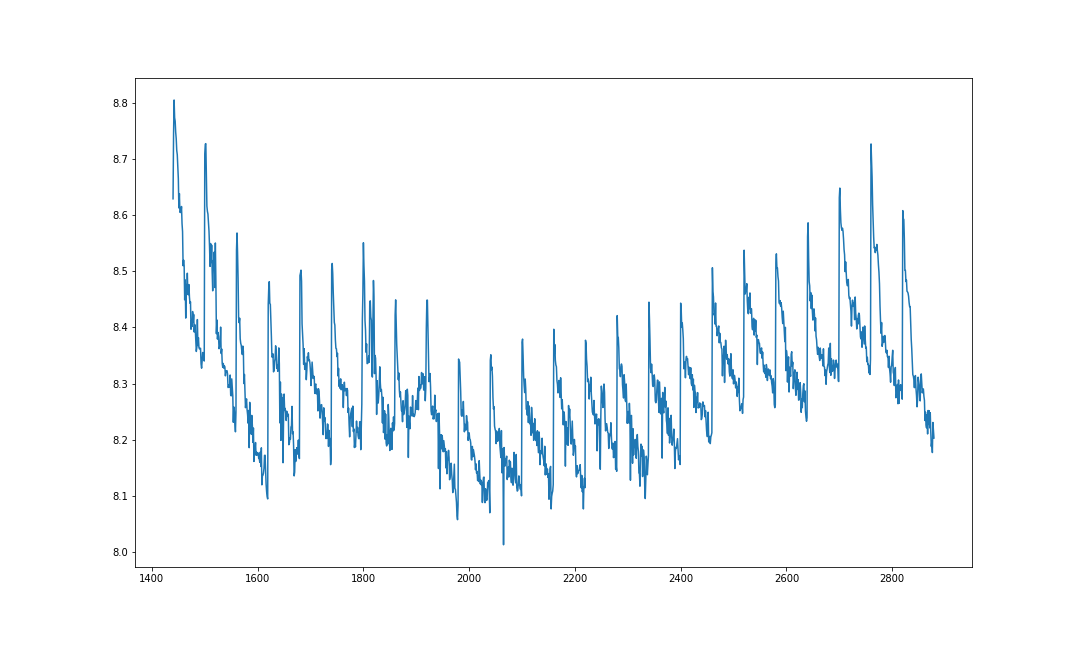
\includegraphics[scale=0.10]{images/010_case_1}
     \end{figure}
\end{frame}

\begin{frame}
    \frametitle{Airpush cases. Fraud elimination}
    \framesubtitle{2. Remove trend}
    \begin{figure}
	\textbf{Clean application}
	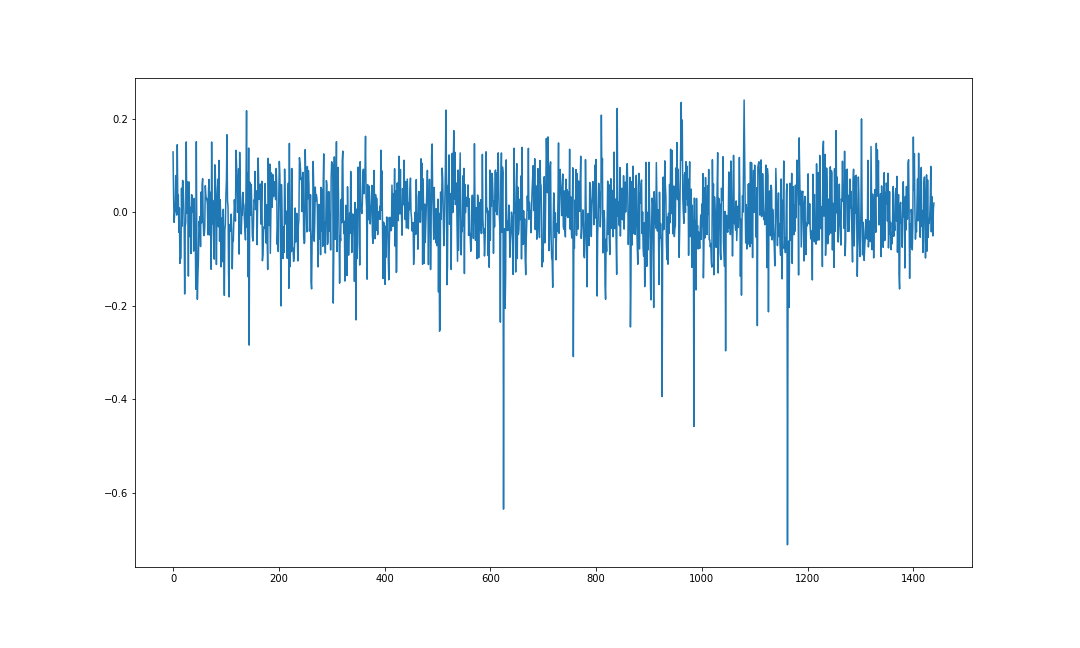
\includegraphics[scale=0.10]{images/011_case_1}
	\textbf{Fraud application}
	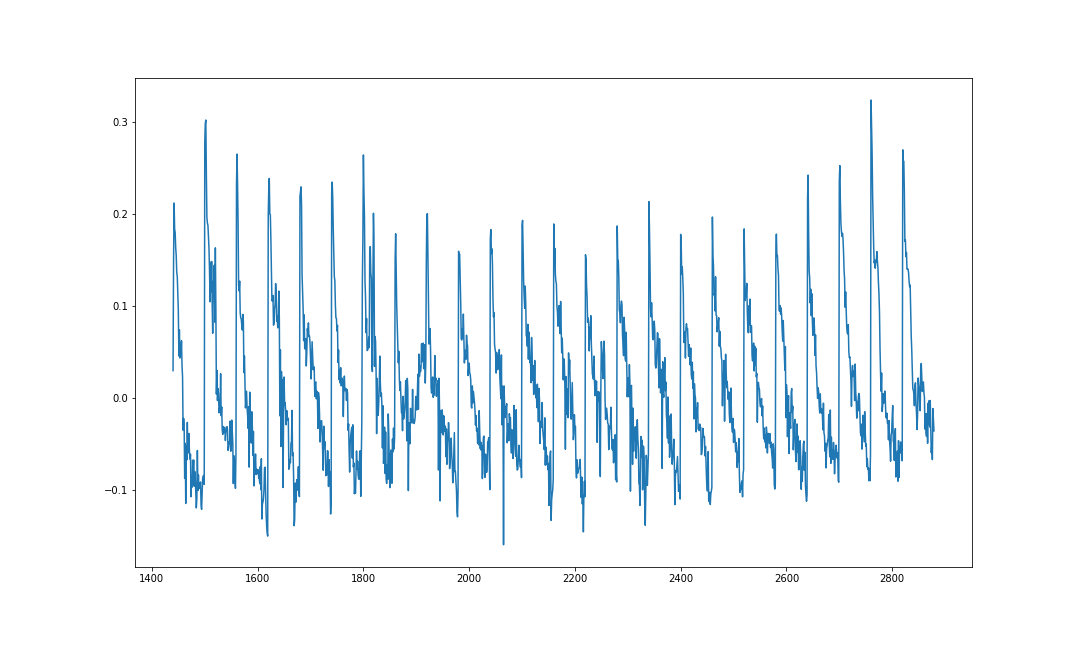
\includegraphics[scale=0.10]{images/012_case_1}
     \end{figure}
\end{frame}

\begin{frame}
    \frametitle{Airpush cases. Fraud elimination}
    \framesubtitle{3. Apply Fourier transform}
    \begin{figure}
	\textbf{Clean application}
	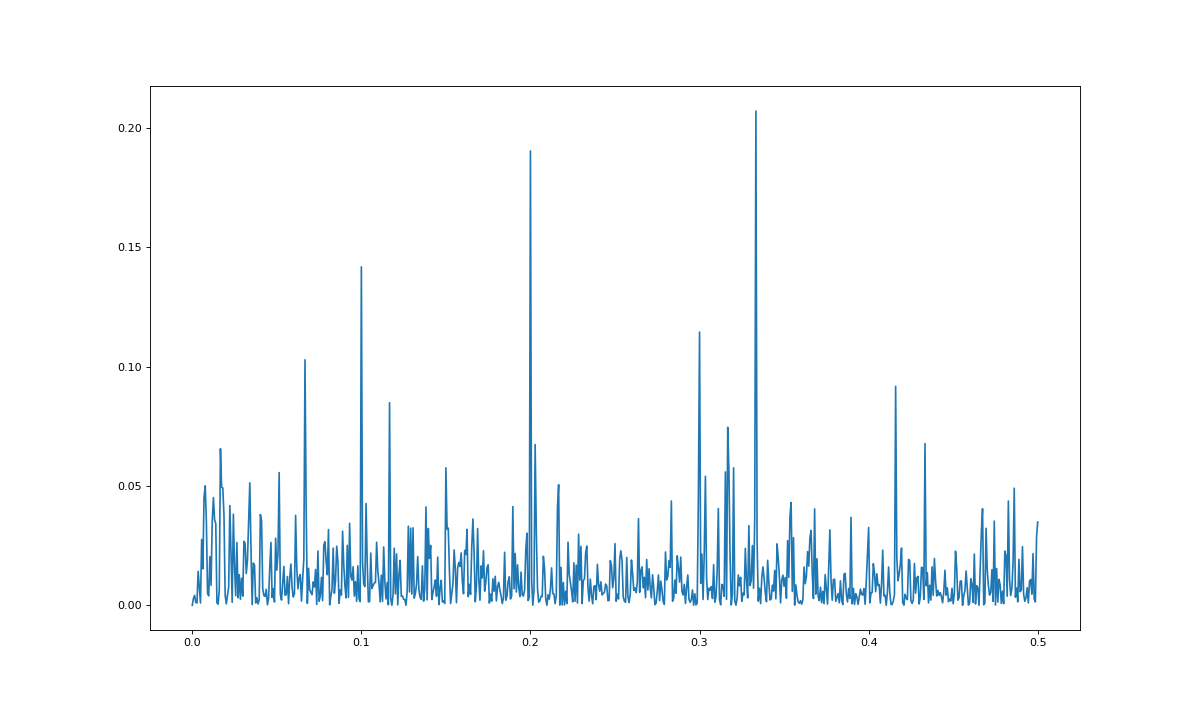
\includegraphics[scale=0.10]{images/013_case_1}
	\textbf{Fraud application}
	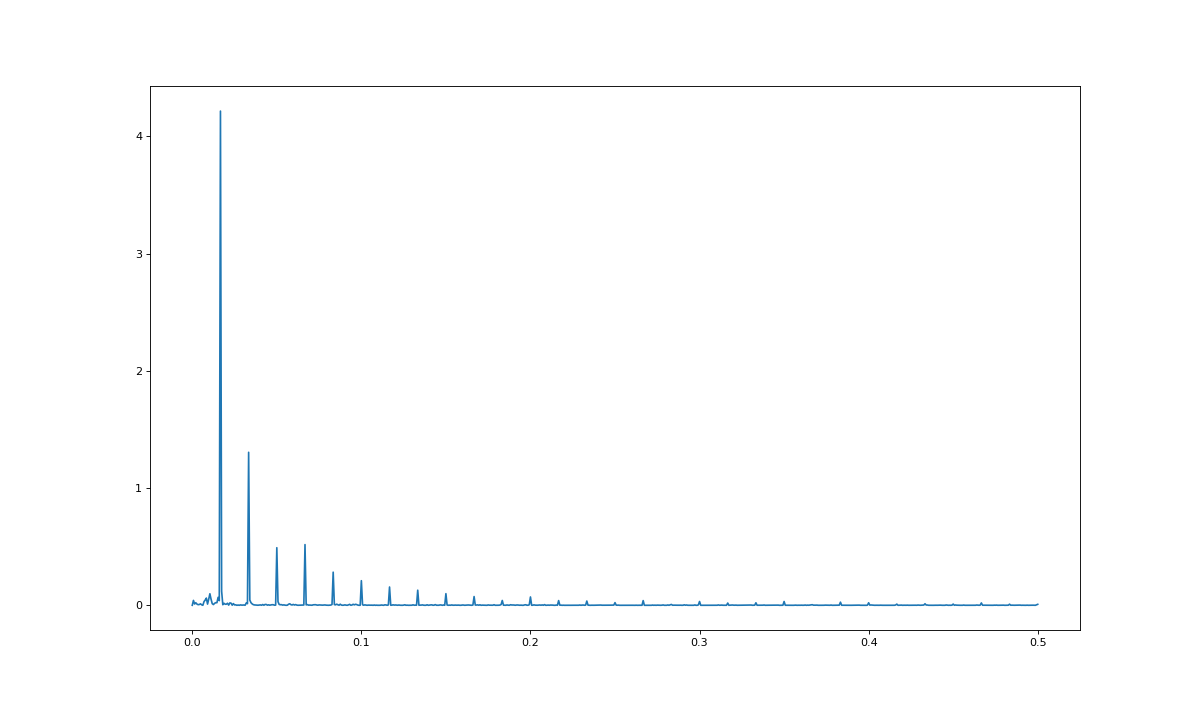
\includegraphics[scale=0.10]{images/014_case_1}
     \end{figure}
\end{frame}

\begin{frame}
    \frametitle{Airpush cases. Fraud elimination}
    \framesubtitle{4. Estimate the distribution of periodogram values}
    \begin{figure}
	\textbf{Clean application}
	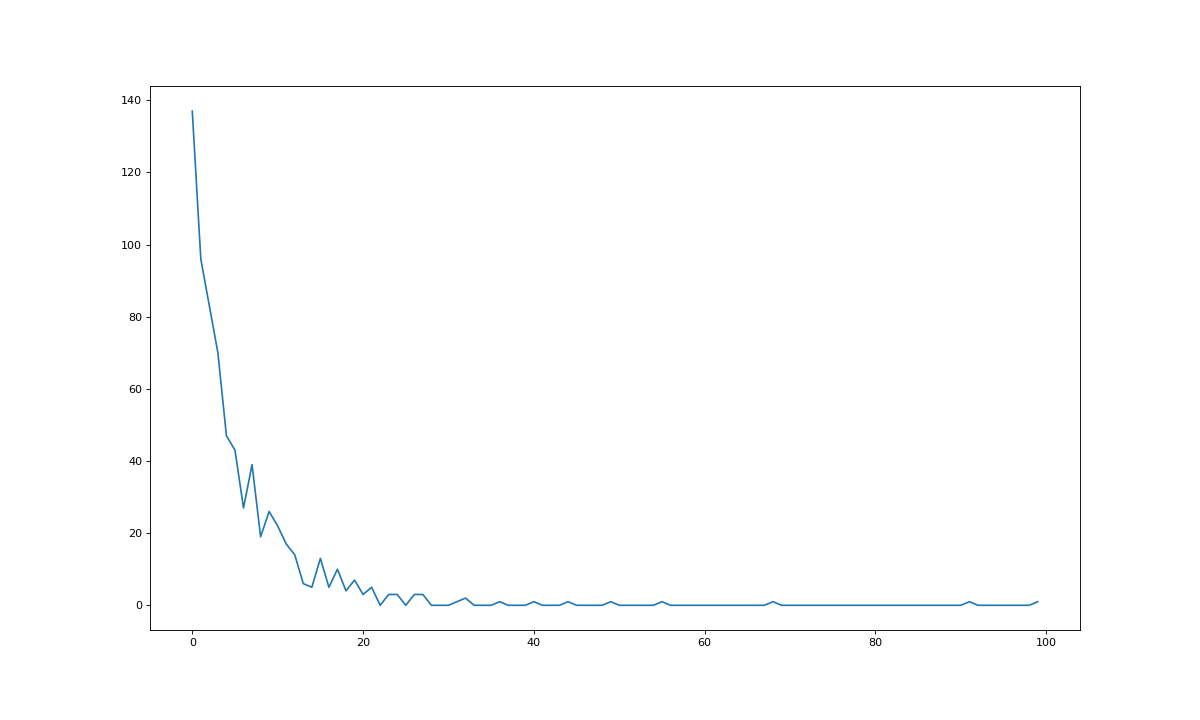
\includegraphics[scale=0.10]{images/015_case_1}
	\textbf{Fraud application}
	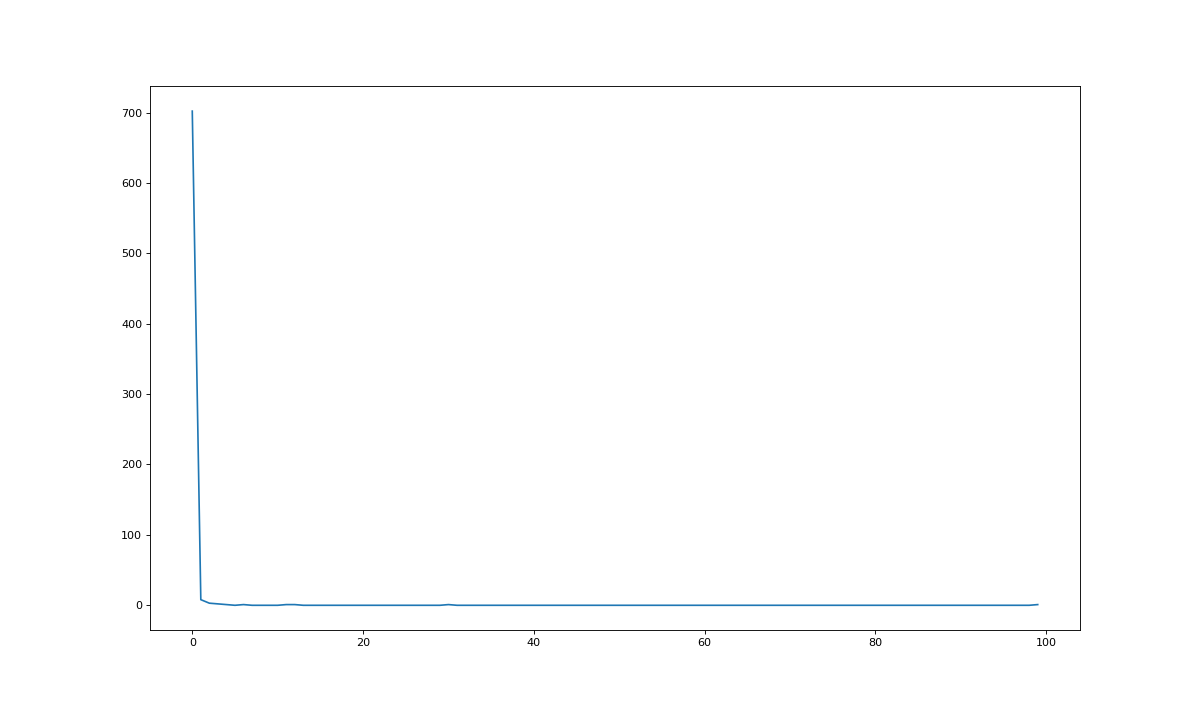
\includegraphics[scale=0.10]{images/016_case_1}
     \end{figure}
\end{frame}

\begin{frame}
    \frametitle{Airpush cases. Fraud elimination}
    \framesubtitle{5. Compare distributions}
    \begin{itemize}
    	\item Clean app score: 0.09
	\item Fraud app score: 1.87
    \end{itemize}
\end{frame}

\end{document}
